\documentclass[a4paper,bibliography=totocnumbered,parskip,headsepline]{scrbook}

\usepackage[utf8]{inputenc}
\usepackage[backend=biber,citestyle=alphabetic,bibstyle=din]{biblatex}
\usepackage[english]{babel}
\usepackage{csquotes}
\usepackage{hyperref}
\usepackage{url}
\usepackage{scrhack}
\usepackage{graphicx}
\usepackage{courier}
\usepackage[T1]{fontenc}
\usepackage{amsmath}
\usepackage[obeyFinal]{todonotes}
\usepackage{multirow}% http://ctan.org/pkg/multirow
\usepackage{listings}
\usepackage{enumitem}
\usepackage[section]{placeins}
\usepackage{tikz}
\usepackage[onehalfspacing]{setspace}
\recalctypearea
\usetikzlibrary{shapes.geometric, arrows}

\lstset{basicstyle=\footnotesize\ttfamily,
        breaklines=true,
%        frame=single,
        language=llvm}

\widowpenalty=1000
\clubpenalty=1000
% Use cite/entry key as fallback label
\DeclareLabelalphaTemplate{
  \labelelement{
    \field[final]{shorthand}
    \field{label}
    \field[strwidth=3,strside=left,ifnames=1]{labelname}
    \field[strwidth=1,strside=left]{labelname}
    \field[final,strwidth=3]{citekey}
  }
  \labelelement{
    \field[strwidth=2,strside=right]{year}
  }
}

% Add labels to bibliography - taken from alphabetic.bbx
\DeclareFieldFormat{labelalphawidth}{\mkbibbrackets{#1}}
\defbibenvironment{bibliography}
  {\list
     {\printtext[labelalphawidth]{%
        \printfield{prefixnumber}%
        \printfield{labelalpha}%
        \printfield{extraalpha}}}
     {\setlength{\labelwidth}{\labelalphawidth}%
      \setlength{\leftmargin}{\labelwidth}%
      \setlength{\labelsep}{\biblabelsep}%
      \addtolength{\leftmargin}{\labelsep}%
      \setlength{\itemsep}{\bibitemsep}%
      \setlength{\parsep}{\bibparsep}}%
      \renewcommand*{\makelabel}[1]{##1\hss}}
  {\endlist}
  {\item}
\DefineBibliographyStrings{english}{%
  bibliography = {References},
}
\bibliography{accelerate}

\newcommand{\executeIffilenewer}[3]{
 \ifnum\pdfstrcmp{\pdffilemoddate{#1}}
 {\pdffilemoddate{#2}}>0
 {\immediate\write18{#3}}\fi
}
\newcommand{\includesvg}[2][]{
 \executeIffilenewer{#2.svg}{#2.pdf}
 {inkscape -z -D --file=#2.svg --export-pdf=#2.pdf}
 \includegraphics[#1]{#2.pdf}
}

\tikzstyle{startstop} = [rectangle, rounded corners, minimum width=3cm, minimum height=1cm,text centered, draw=black, fill=red!30]
\tikzstyle{io} = [trapezium, trapezium left angle=70, trapezium right angle=110, minimum width=3cm, minimum height=1cm, text centered, draw=black, fill=blue!30]
\tikzstyle{process} = [rectangle, minimum width=3cm, minimum height=1cm, text centered, draw=black, fill=orange!30]
\tikzstyle{decision} = [diamond, minimum width=3cm, minimum height=1cm, text centered, draw=black, fill=green!30]
\tikzstyle{arrow} = [thick,->,>=stealth]

\showboxdepth=\maxdimen
\showboxbreadth=\maxdimen
\begin{document}

\frontmatter

\begin{titlepage}

\begin{center}
{\huge \textit{Master Thesis}}

\vspace{2cm}

{\Large \textbf{Generating LLVM IR using \\Template Meta Programming in Haskell}}

\vspace{1.75cm}

\vspace{1.75cm}

{\large Christian-Albrechts-Universität zu Kiel\\
   Department of Computer Science\\
   Programming Languages and Compiler Construction
}

\end{center}

\vspace{2cm}

\begin{tabular}{ll}
student: & \textbf{Timo von Holtz} \\
\multirow{2}{*}{advised by:} & Priv.-Doz. Dr. Frank Huch\\
 & Assoc. Prof. Dr. Manuel M. T. Chakravarty
\end{tabular}

\vspace{1cm}

\begin{center}
Kiel, \today
\end{center}

\end{titlepage}

\chapter*{Selbstständigkeitserklärung}

Ich erkläre hiermit, dass ich die vorliegende Arbeit selbstständig und nur unter Verwendung der angegebenen Literatur und Hilfsmittel angefertigt habe.


\today
\begin{flushright}
\rule{6cm}{0.4pt} \\
Timo von Holtz
\end{flushright}
\clearpage
% oder auch manuell

\chapter*{Abstract}
Implementing parallel computations is traditionally done in low level languages like C or FORTRAN.
This allows great control over the details of execution.
Unfortunately, this also comes with the complexities of using a low-level language.
To make this easier, \citeauthor{chakravarty2011accelerating} have developed Accelerate, an embedded array language for computations for high-performance computing in Haskell.
The main execution target of this EDSL is GPUs via CUDA.

\citeauthor{trevor2014llvm} started working on an alternative implementation using LLVM.
I contribute to this work by implementing a different approach to code-generation for LLVM using quasi-quotation.
I use this quasi-quoter to implement the skeletons in the LLVM backend.

% Verzeichnisse
\listoftodos
\tableofcontents   % Inhaltsverzeichnis
\listoffigures     % Abbildungsverzeichnis
\listoftables      % Tabellenverzeichnis
\mainmatter

\chapter{Introduction}
Processing large amounts of data is becoming more and more important.
To meet this demand, there have been a number of approaches.
Since the continuous improvement in speed predicted by Moore's law is no longer possible, newer architectures rely on many parallel cores instead of one.
This comes at a cost however, as it is no longer possible to use all the power given just by implementing a sequential algorithm.

Most computing-intense calculations can be expressed as operations on arrays.
This class of problems is addressed by Accelerate\cite{chakravarty2011accelerating,mcdonelloptimising}.
Accelerate is an an embedded array language for computations for high-performance computing in Haskell.

The way an algorithm is expressed in Accelerate is using a set of combinator functions like \lstinline[language=haskell]!map! or \lstinline[language=haskell]!fold!.
To give an example, lets look at the dot product of 2 vectors.
\[
\begin{pmatrix}
x_0 \\ ... \\ x_{n-1}
\end{pmatrix}
\times
\begin{pmatrix}
y_0 \\ ... \\ y_{n-1}
\end{pmatrix}
= \displaystyle\sum_{i=0}^{n-1} x_i*y_i
\]

This can be trivially implemented in Haskell using \lstinline[language=haskell]!foldl'!\footnote{The implementation of \lstinline[language=haskell]!foldl! in Haskell is such, that it will produce large intermediate chunks. \lstinline[language=haskell]!foldl'! is a strict variant, so this doesn't happen.} and \lstinline[language=haskell]!zipWith!.
\begin{lstlisting}[language=haskell]
dotp_list :: [Float] -> [Float] -> Float
dotp_list xs ys =
  foldl (+) 0 (zipWith (*) xs ys)
\end{lstlisting}
This code is purely sequential however and is therefore limited to only one CPU.
Accelerate allows you to write this computation in nearly exactly the same way.
\begin{lstlisting}[language=haskell]
dotp :: Acc (Vector Float)
     -> Acc (Vector Float)
     -> Acc (Scalar Float)
dotp xs ys = fold (+) 0 (zipWith (*) xs ys)
\end{lstlisting}
To run this computation however, there has to be some parallel implementation.
The implementation presented in the original Accelerate work targets NVIDIA GPUs using CUDA, as those offered the most performance, while being traditionally hard to program.
While this is good in a specialized setting where there is a powerful GPGPU available, it is not suitable to accelerate computations on any given machine.
To use Accelerate in a more general setting, there has been early work on an alternative backend to Accelerate using LLVM.\cite{trevor2014llvm}
This work includes both a CPU and a GPU backend.
In this thesis I will develop a novel approach to code generation for LLVM.
I will use this to implement the missing pieces in the code generation of the native LLVM backend.


\chapter{Technologies}
Before I 

\section{LLVM}
LLVM\cite{lattner2002llvm} is a compiler infrastructure written in C++.
In contrast to GCC it is designed to be used as a library by compilers.
Originally implemented for C and C++, the language-agnostic design (and the success) of LLVM has since spawned a wide variety of front ends: languages with compilers that use LLVM include ActionScript, Ada, D, Fortran, OpenGL Shading Language, Haskell, Java bytecode, Julia, Objective-C, Python, Ruby, Rust, Scala and C.

\subsection{LLVM IR}
LLVM defines it's own language to represent programs.
It uses Static Single Assignment (SSA) form.\cite{alpern1988detecting,rosen1988global}
A program is said to be in SSA form if each of its variables is defined exactly once, and each use of a variable is dominated by that variable’s definition.
SSA form greatly simplifies many dataflow optimizations because only a single definition can reach a particular use of a value, and finding that definition is trivial.

To get idea of how this looks like in practice, let's look at an example.
Figure \ref{fig:sumc} shows a simple C function to sum up the elements of an array. The corresponding LLVM code is shown in figure \ref{fig:sumll}.

\begin{figure}
\begin{lstlisting}[language=C]
int sum(int* a, int length) {
  int x = 0;
  for (int i=0;i<length;i++) {
    x += a[i];
  }
  return x;
}
\end{lstlisting}
\caption{sum as a C function}
\label{fig:sumc}
\end{figure}

\begin{figure}
\begin{lstlisting}
define i32 @sum(i32* nocapture readonly %a, i32 %length) {
entry:
  %cmp4 = icmp sgt i32 %length, 0
  br i1 %cmp4, label %for.body, label %for.end

for.body:                                         ; preds = %entry, %for.body
  %indvars.iv = phi i64 [ %indvars.iv.next, %for.body ], [ 0, %entry ]
  %x.05 = phi i32 [ %add, %for.body ], [ 0, %entry ]
  %arrayidx = getelementptr inbounds i32* %a, i64 %indvars.iv
  %0 = load i32* %arrayidx, align 4
  %add = add nsw i32 %0, %x.05
  %indvars.iv.next = add nuw nsw i64 %indvars.iv, 1
  %lftr.wideiv = trunc i64 %indvars.iv.next to i32
  %exitcond = icmp eq i32 %lftr.wideiv, %length
  br i1 %exitcond, label %for.end, label %for.body

for.end:                                          ; preds = %for.body, %entry
  %x.0.lcssa = phi i32 [ 0, %entry ], [ %add, %for.body ]
  ret i32 %x.0.lcssa
}
\end{lstlisting}
\caption{sum as a LLVM}
\label{fig:sumll}
\end{figure}

The first obvious difference is the lack of sophisticated control structures.
In LLVM every function is divided into basic blocks.
A basic block is a continuous stream of instructions with a terminator at the end.
Instructions are add, mult, call, \dots, but also call.
Terminators can either be used to jump to another block (branch) or return to the calling function.

To allow for dynamic control flow, there are $\Phi$-nodes.
These specify the the value of a new variable depending on what the last block was.
The $\Phi$-nodes in the SSA are represented with \lstinline{phi}-instructions.
In LLVM, these have to preceed every other instruction in a given basic block.

\subsubsection{Types}
The LLVM type system is one of the most important features of the intermediate representation.
Being typed enables a number of optimizations to be performed directly, without having to do extra analyses on the side before the transformation.

Important Types are:
\begin{itemize}[noitemsep]
\item[-] \lstinline{void}, which represents no value
\item[-] integers with specified length N: \lstinline{iN}
\item[-] floating point numbers: \lstinline{half, float, double, ...}
\item[-] pointers: \lstinline{<type> *}
\item[-] function types: \lstinline{<returntype> (<parameter list>)}
\item[-] vector types: \lstinline{< <# elements> x <elementtype> >}
\item[-] array types: \lstinline{[<# elements> x <elementtype>]}
\item[-] structure types: \lstinline!{ <type list> }!
\end{itemize}

\subsection{Vectorization}
Modern CPUs all have SIMD units to execute an instruction on multiple datasets in parallel.
Usind these units is easy with LLVM.
All operations (\lstinline{add}, \lstinline{fadd}, \lstinline{sub}, \dots) can be used with vector arguments the same way as with scalar arguments.

To manually exploit this can be tricky however.
LLVM has multiple strategies to fuse similar instructions or tight inner loops into vectorized code.\cite{llvmauto}

\subsubsection{Loop Vectorizer}
The Loop Vectorizer tries to vectorize tight inner loops.
To get an idea of how these work, lets look at the example from figure \ref{fig:sumc}.
To build the sum, every element of the array is added to an accumulator.
Since addition is associative and commutative, the additions can be reordered.
Given a vector width of 2, the sum of $2*n$ and $2*n+1$ are calculated in parallel and then added together.
In addition to this, the vectorizer will also unroll the inner loop to make fewer jumps necessary.
Figure \ref{fig:sumllvec} shows the corresponding llvm code without loop unroll, as this increases code size dramatically.

\begin{figure}
\begin{lstlisting}[basicstyle=\scriptsize\ttfamily]
define i32 @sum(i32* nocapture readonly %a, i32 %length) {
entry:
  %cmp4 = icmp sgt i32 %length, 0
  br i1 %cmp4, label %for.body.preheader, label %for.end

for.body.preheader:                   ; preds = %entry
  %0 = add i32 %length, -1
  %1 = zext i32 %0 to i64
  %2 = add i64 %1, 1
  %end.idx = add i64 %1, 1
  %n.vec = and i64 %2, 8589934590
  %cmp.zero = icmp eq i64 %n.vec, 0
  br i1 %cmp.zero, label %middle.block, label %vector.body

vector.body:                          ; preds = %for.body.preheader, %vector.body
  %index = phi i64 [ %index.next, %vector.body ], [ 0, %for.body.preheader ]
  %vec.phi = phi <2 x i32> [ %5, %vector.body ],
                           [ zeroinitializer, %for.body.preheader ]
  %3 = getelementptr inbounds i32* %a, i64 %index
  %4 = bitcast i32* %3 to <2 x i32>*
  %wide.load = load <2 x i32>* %4, align 4
  %5 = add nsw <2 x i32> %wide.load, %vec.phi
  %index.next = add i64 %index, 2
  %6 = icmp eq i64 %index.next, %n.vec
  br i1 %6, label %middle.block, label %vector.body

middle.block:                         ; preds = %vector.body, %for.body.preheader
  %resume.val = phi i64 [ 0, %for.body.preheader ], [ %n.vec, %vector.body ]
  %rdx.vec.exit.phi = phi <2 x i32> [ zeroinitializer, %for.body.preheader ],
                                    [ %5, %vector.body ]
  %rdx.shuf = shufflevector <2 x i32> %rdx.vec.exit.phi, <2 x i32> undef,
                                                         <2 x i32> <i32 1, i32 undef>
  %bin.rdx = add <2 x i32> %rdx.vec.exit.phi, %rdx.shuf
  %7 = extractelement <2 x i32> %bin.rdx, i32 0
  %cmp.n = icmp eq i64 %end.idx, %resume.val
  br i1 %cmp.n, label %for.end, label %for.body

for.body:                             ; preds = %middle.block, %for.body
  %indvars.iv = phi i64 [ %indvars.iv.next, %for.body ], [ %resume.val, %middle.block ]
  %x.05 = phi i32 [ %add, %for.body ], [ %7, %middle.block ]
  %arrayidx = getelementptr inbounds i32* %a, i64 %indvars.iv
  %8 = load i32* %arrayidx, align 4
  %add = add nsw i32 %8, %x.05
  %indvars.iv.next = add nuw nsw i64 %indvars.iv, 1
  %lftr.wideiv = trunc i64 %indvars.iv.next to i32
  %exitcond = icmp eq i32 %lftr.wideiv, %length
  br i1 %exitcond, label %for.end, label %for.body

for.end:                              ; preds = %for.body, %middle.block, %entry
  %x.0.lcssa = phi i32 [ 0, %entry ], [ %add, %for.body ], [ %7, %middle.block ]
  ret i32 %x.0.lcssa
}
\end{lstlisting}
\caption{Vectorized Sum}
\label{fig:sumllvec}
\end{figure}

Apart from reductions, LLVM can also vectorize the following:
\begin{itemize}[noitemsep]
 \item[-] Loops with unknown trip count
 \item[-] Runtime Checks of Pointers
 \item[-] Reductions
 \item[-] Inductions
 \item[-] If Conversion
 \item[-] Pointer Induction Variables
 \item[-] Reverse Iterators
 \item[-] Scatter / Gather
 \item[-] Vectorization of Mixed Types
 \item[-] Global Structures Alias Analysis
 \item[-] Vectorization of function calls
 \item[-] Partial unrolling during vectorization
\end{itemize}
A detailed description can be found at \citeurl{llvmauto}

\subsubsection{SLP Vectorizer}
The goal of SLP vectorization (a.k.a. superword-level parallelism) is to combine similar independent instructions into vector instructions.
Memory accesses, arithmetic operations, comparison operations, PHI-nodes, can all be vectorized using this technique.
For example, the following function performs very similar operations on its inputs (a1, b1) and (a2, b2).

\begin{lstlisting}[language=C]
void foo(double a1, double a2, double b1, double b2, double *A) {
  A[0] = a1*(a1 + b1)/b1 + 50*b1/a1;
  A[1] = a2*(a2 + b2)/b2 + 50*b2/a2;
}
\end{lstlisting}

The SLP vectorizer may combine these into vector operations.
Figures \ref{fig:slpll1} and \ref{fig:slpll2} show the the corresponding LLVM before and after SLP vectorization.

\begin{figure}
\begin{lstlisting}
define void @foo(double %a1, double %a2, double %b1, double %b2, double* %A) {
entry:
  %add = fadd double %a1, %b1
  %mul = fmul double %add, %a1
  %div = fdiv double %mul, %b1
  %mul1 = fmul double %b1, 5.000000e+01
  %div2 = fdiv double %mul1, %a1
  %add3 = fadd double %div, %div2
  store double %add3, double* %A, align 8
  %add4 = fadd double %a2, %b2
  %mul5 = fmul double %add4, %a2
  %div6 = fdiv double %mul5, %b2
  %mul7 = fmul double %b2, 5.000000e+01
  %div8 = fdiv double %mul7, %a2
  %add9 = fadd double %div6, %div8
  %arrayidx10 = getelementptr inbounds double* %A, i64 1
  store double %add9, double* %arrayidx10, align 8
  ret void
}
\end{lstlisting}
\caption{\lstinline{foo} without SLP vectorization}
\label{fig:slpll1}
\end{figure}

\begin{figure}
\begin{lstlisting}
define void @foo(double %a1, double %a2, double %b1, double %b2, double* %A) {
entry:
  %0 = insertelement <2 x double> undef, double %a1, i32 0
  %1 = insertelement <2 x double> %0, double %a2, i32 1
  %2 = insertelement <2 x double> undef, double %b1, i32 0
  %3 = insertelement <2 x double> %2, double %b2, i32 1
  %4 = fadd <2 x double> %1, %3
  %5 = fmul <2 x double> %4, %1
  %6 = fdiv <2 x double> %5, %3
  %7 = fmul <2 x double> %3, <double 5.000000e+01, double 5.000000e+01>
  %8 = fdiv <2 x double> %7, %1
  %9 = fadd <2 x double> %6, %8
  %10 = bitcast double* %A to <2 x double>*
  store <2 x double> %9, <2 x double>* %10, align 8
  ret void
}
\end{lstlisting}
\caption{\lstinline{foo} with SLP vectorization}
\label{fig:slpll2}
\end{figure}

\subsubsection{Fast-Math Flags}
In order for the Loop vectorizer to work, the operations involved need to be associative.
When dealing with floating point numbers, the basic operations like \lstinline{fadd} and \lstinline{fmul} don't satisfy this condition.
To vectorize the code regardless, LLVM has the notion of fast-math-flags.
These tell the optimizer to assume certain properties that aren't true in general.

Available flags are\cite{llvmref}:
\begin{itemize}
\item[nnan] No NaNs - Allow optimizations to assume the arguments and result are not NaN. Such optimizations are required to retain defined behavior over NaNs, but the value of the result is undefined.
\item[ninf] No Infs - Allow optimizations to assume the arguments and result are not +/-Inf. Such optimizations are required to retain defined behavior over +/-Inf, but the value of the result is undefined.
\item[nsz] No Signed Zeros - Allow optimizations to treat the sign of a zero argument or result as insignificant.
\item[arcp] Allow Reciprocal - Allow optimizations to use the reciprocal of an argument rather than perform division.
\item[fast] Fast - Allow algebraically equivalent transformations that may dramatically change results in floating point (e.g. reassociate). This flag implies all the others.
\end{itemize}

\subsection{llvm-general}
To use LLVM from Haskell, there are multiple options.
The most complete is llvm-general.\cite{scarlet2013llvm}
Instead of exposing the LLVM API directly, it uses an ADT to represent LLVM IR.
This can then be translated into the corresponding C++ object.
It also supports the other way, transforming the object back into the ADT.

Using an ADT instead of writing directly to the C++ object has many advantages.
This way, the code can be produced and manipulated outside the IO context.
It is also much easier to reason about within Haskell.

llvm-general also supports optimization and jit-compilation.
The optimization is controlled by a \lstinline[language=haskell]!PassSetSpec!
This offers the user 2 different options: \lstinline[language=haskell]!CuratedPassSetSpec! and \lstinline[language=haskell]!PassSetSpec!.
Using \lstinline[language=haskell]!CuratedPassSetSpec! is the easier option of the 2.
It offers a similar level of control as specifying \texttt{-On} at the command line.
Using \lstinline[language=haskell]!PassSetSpec! gives much more control over the exact passes run, but you have to specify them one by one.
Both of these specs also come with fields to specify information about the target.

\section{Accelerate}
Accelerate\cite{chakravarty2011accelerating,mcdonelloptimising} is an an embedded array language for computations for high-performance computing in Haskell.
Computations on multi-dimensional, regular arrays are expressed in the form of parameterised collective operations, such as maps, reductions, and permutations.
It is very similar to Repa\cite{keller2010regular} in the way computations are specified.
The difference is in the way the computation gets evaluated.
While Repa produces its result immediately, Accelerate collects the computation which can then be executed.
This approach is necessaray, as Accelerate isn't limited to be run on a CPU.
The main back-end of accelerate is in fact based on CUDA.

\subsection{Usage}
To give an example of how to use Accelerate, lets look at the dot product of 2 vectors.
This could easily implemented in Haskell like this.

\begin{lstlisting}[language=haskell]
dotp_list :: [Float] -> [Float] -> Float
dotp_list xs ys = foldl (+) 0 (zipWith (*) xs ys)
\end{lstlisting}

You can write nearly exactly the same function in Accelerate:

\begin{lstlisting}[language=haskell]
dotp :: Acc (Vector Float)
     -> Acc (Vector Float)
     -> Acc (Scalar Float)
dotp xs ys = fold (+) 0 (zipWith (*) xs ys)
\end{lstlisting}

The first is the difference is the use of a different datastructure.
A \lstinline[language=haskell]!Vector! is an \lstinline[language=haskell]!Array! with one dimension.
Similarly, a \lstinline[language=haskell]!Scalar! is an \lstinline[language=haskell]!Array! with 0 dimensions.
These are then wrapped in the \lstinline[language=haskell]!Acc! type.
\lstinline[language=haskell]!Acc a! is a computation, that yields an \lstinline[language=haskell]!a!.

The second difference is the \lstinline[language=haskell]!fold!.
Unlike the \lstinline[language=haskell]!foldl! in the Haskell example, this \lstinline[language=haskell]!fold! doesn't specify the order of operations.
This is important as it allows for an efficient implementation.
In order of this to work, the operation passed to \lstinline[language=haskell]!fold! has to be associative.

If we want to call this function, we have to somehow produce values of type \lstinline[language=haskell]!Acc (Vector Float)!.

First the list is converted with \lstinline[language=haskell]!fromList!.
To see what it does, lets first look at its type.

\begin{lstlisting}[language=haskell]
fromList :: (Elt e, Shape sh) => sh -> [e] -> Array sh e
\end{lstlisting}

In addition to the list of elements, \lstinline[language=haskell]!fromList! takes the shape of the resulting \lstinline[language=haskell]!Array!.
Shapes can have an arbitrary amount of dimensions, but in this case it is only one.
To construct a shape, there are 2 datatypes:

\begin{lstlisting}[language=haskell]
data Z = Z
data tail :. head = tail :. head
\end{lstlisting}

The head in this case represents the innermost dimension.
The tail has to also be a shape.

With this, we get
\begin{lstlisting}[language=haskell]
type DIM0 = Z
type DIM1 = DIM0 :. Int
type DIM2 = DIM1 :. Int
...
\end{lstlisting}
and
\begin{lstlisting}[language=haskell]
type Scalar a = Array DIM0 a
type Vector a = Array DIM1 a
\end{lstlisting}

To lift the Arrays we get via \lstinline[language=haskell]!fromList! we use the function
\begin{lstlisting}[language=haskell]
use :: Arrays arrays => arrays -> Acc arrays
\end{lstlisting}

This is all we need to call \lstinline[language=haskell]!dotp!.

\begin{lstlisting}[language=haskell]
dotp' :: [Float] -> [Float] -> Acc (Scalar Float)
dotp' xs ys =
  let  xs' = use (fromList (Z :.length xs) xs)
       ys' = use (fromList (Z :.length xs) ys)
  in dotp xs' ys'
\end{lstlisting}

But we still only have the computation.
To get the result out of the computation, we have to \lstinline[language=haskell]!run! it.
After that we can convert the \lstinline[language=haskell]!Array! back to a list and extract the element.

\begin{lstlisting}[language=haskell]
dotp_list1 :: [Float] -> [Float] -> Float
dotp_list1 xs ys = head . toList $ run $ (dotp' xs ys)
\end{lstlisting}

\subsection{Representation}
Accelerate represents its arrays internally as regular unboxed one-dimensional arrays.
In addition to this, the lengths of each dimension is stored.
In case of a matrix, this would be height and width.

Rather than just simple types like \lstinline[language=haskell]!Int! or \lstinline[language=haskell]!Float!, Accelerate also supports tuples as elements
These cannot be easily stored in an unboxed array.
Instead, arrays of tuples are stored as tuples of arrays.

\begin{lstlisting}[language=haskell]
Vector (Int, Float) ~ (Vector Int, Vector Float)
\end{lstlisting}

\subsection{Skeletons}
To execute any computation on a given architecture, the involved functions like \lstinline[language=haskell]!fold! or \lstinline[language=haskell]!map! have to be implemented.
This is easy if the target is Haskell.
The reason however that it is easy is the fact, that Haskell has support for higher-level functions like \lstinline[language=haskell]!fold! and \lstinline[language=haskell]!map!.
In C, this can be emulated by using function pointers.
This approach however is not very performant if the function is relatively simple as it involves multiple jumps and the manipulation of the call stack.

Accelerate uses skeletons instead.
The idea is to write the function as you would normally, but leave blanks for the concrete types and passed function.
When needed it can then be instantiated with the correct types and function.
Figure \ref{fig:mapskelC} illustrates the idea using \lstinline[language=haskell]!map!.

\begin{figure}
\begin{lstlisting}[language=C]
void map
(
  TyOut *           d_out,
  const TyIn *      d_in,
  const int         length
){
  for (int i=0; i < length; ix += 1) {
    d_out[i] = apply(d_in[i]);
  }
}
\end{lstlisting}
\caption{\lstinline[language=haskell]!map! Skeleton in C}
\label{fig:mapskelC}
\end{figure}

Instead of the single array for input and output however, there will often be multiple.
This is because a singe array in Accelerate be represented by multiple arrays internally.

\subsection{Fusion}
Consider the following example from earlier.

\begin{lstlisting}[language=haskell]
dotp xs ys = fold (+) 0 (zipWith (*) xs ys)
\end{lstlisting}

This can be rewritten as

\begin{lstlisting}[language=haskell]
dotp xs ys =
  let zs = zipWith (*) xs ys
  in fold (+) 0 zs
\end{lstlisting}

First, the elements of the 2 arrays are combined pair-wise using \lstinline[language=haskell]!zipWith! and stored in a temporary array.
As a second step, these elements are then combined into a \lstinline[language=haskell]!Scalar! using \lstinline[language=haskell]!fold!.
Although this works perfectly well, it produces an intermediate array.
This means additional writes and reads from memory.
Considering that memory access is very costly this should better be avoided.

The solution is to delay the computation of the intermediate array.
This means, that instead of computing the array in memory, it is done on-the-fly.
This changes the construction of the skeletons somewhat.
Instead of declaring the inputs directly, the arrays needed are passed in as an array environment.
This is then accessed through a function \lstinline[language=haskell]!delayedLinearIndex!.

\subsection{LLVM Backend}
Apart from the CUDA-backend and the Interpreter, There are a number of incomplete backends for Accelerate.
One of those that looks promising is the LLVM backend.\cite{trevor2014llvm}
It uses llvm-general to bind to the LLVM API.
It supports both CPUs as well as NVIDIA GPUs through PTX.
In contrast to the CUDA backend, this has the advantage that no external program has to be called for compilation of the kernels.
This is also true for the CPU side.
Unfortunately, it is not possible to ``write once, run everywhere'' with LLVM.
Although the instructions are exactly the same between architectures, the supplied libraries are not.
That is why the Skeletons cannot be shared between the 2.

To run a computation in the LLVM native backend, the skeletons are first optimized and compiled to a callable function.
Similar to repa, it uses uses gang workers\cite{chakravarty2007data} for execution.
These are multiple threads, typically as many as there are capabilities available.
They wait on an \lstinline[language=haskell]!MVar! for IO actions to perform.
At first, the load is split evenly between the workers.
If a thread finishes early however, it looks for more work.
If it finds that another thread has excess work available, it will steal half of it.
This process is called work stealing.
On a shared memory architecture, this has very little overhead.

In this thesis, I will mainly work on the native backend, but the results should be transferable to the PTX backend as well.

\section{Template Haskell}
Template Haskell is an extension to Haskell that allows you to do type-safe compile-time meta-programming, with Haskell both as the manipulating language and the language being manipulated.
Pre-7.8, one would get a Template Haskell expression using quasiquoters like this.
\begin{lstlisting}[language=haskell]
foo :: Q Exp
foo = [|Just 5|]
\end{lstlisting}
It is not clear which type of expression it is.
Another nasty side-effect of this is that the expression is not checked to be consistent internally.
That leads to something like this being legal.
\begin{lstlisting}[language=haskell]
bar :: Q Exp
bar = [|case 1 of
          Nothing -> 42
          True    -> ()|]
\end{lstlisting}
Apart from being syntactically correct, this makes no sense at all.
With GHC 7.8, a new form of quoting Haskell code was introduced.
\begin{lstlisting}[language=haskell]
foo :: Q (TExp (Maybe Int))
foo = [||Just 5||]
\end{lstlisting}
The code is now typechecked along with the rest of the code in the module.
This means it is no longer possible to easily produce nearly untraceable type errors with Template Haskell.
The structure of the expressions remains unchanged however.
\begin{lstlisting}[language=haskell]
newtype TExp a = TExp { unType :: Exp }
\end{lstlisting}
This means it is possible to use typed expressions in places where untyped an untyped expression is exprected.
The reverse is also true, but type safety is lost in the process.
\begin{lstlisting}[language=haskell]
unsafeTExpCoerce :: Q Exp -> Q (TExp a)
\end{lstlisting}
To use the defined expression, it can then be spliced in using \lstinline[language=haskell]{$$(..)}.

This, however, is not possible everywhere.
The following for example is not legal.
\begin{lstlisting}[language=haskell]
bar :: Int
bar = let x = [||1||]
      in $$(x)
\end{lstlisting}
And produces this error message:
\begin{verbatim}
GHC stage restriction:
  'x' is used in a top-level splice or annotation,
  and must be imported, not defined locally
In the splice: $$x
\end{verbatim}
Template Haskell code has to be executable on compile-time.
This means that in a splice, all expressions must be known.
As a consequence, they can't be defined locally or passed in as function arguments.
Not having this restriction would lead to Haskell not being type safe.

\chapter{Contributions}
Before we look at the intricate details I want to summarize the contributions I made.
First is of course my approach to generate LLVM code via template meta programming.
While working with accelerate-llvm, I discovered a few additional obstacles however, which I will also present here.

\section{llvm-general-quote}
When writing a compiler using LLVM in Haskell there is a good tutorial on how to do it at \citeurl{diehl2014jit}.
It uses \citetitle{scarlet2013llvm} to interface with LLVM.
The Idea followed in this tutorial is to use a monadic generator to produce the AST.
The goal of monadic code generation is to use the state of the monad to store the instructions.

Figure \ref{fig:formonad} shows how to implement a simple for loop using monadic generators.
\begin{figure}
\begin{lstlisting}[language=haskell]
for :: Type                             -- type of the index
    -> Operand                          -- starting index
    -> (Operand -> CodeGen Operand)     -- loop test to keep going
    -> (Operand -> CodeGen Operand)     -- increment the index
    -> (Operand -> CodeGen ())          -- body of the loop
    -> CodeGen ()
for ti start test incr body = do
  loop  <- newBlock "for.top"
  exit  <- newBlock "for.exit"

  -- entry test
  c    <- test start
  top  <- cbr c loop exit

  -- Main loop
  setBlock loop
  c\_i <- freshName
  let i = local c\_i

  body i

  i'   <- incr i
  c'   <- test i'
  bot  <- cbr c' loop exit
  \_    <- phi loop c\_i ti [(i',bot), (start,top)]

  setBlock exit
\end{lstlisting}
\caption{Monadic generation of for loop}
\label{fig:formonad}
\end{figure}

Unfortunately, this produces a lot of boilerplate code.
We have to define the basic blocks manually and add the instructions one by one.
This has some obvious drawbacks, as the code can get unreadable pretty quickly.

A more clean approach is to use a complete EDSL.
The idea here is to use block structure to specify the individual elements.
An implementation of this idea is \citetitle{nathan2014llvm}.
It actually goes further, as it also typechecks the produced code.

I propose a third approach using quasiquotation\cite{mainland2007quote}.
The idea behind quasiquotation is, that you can define a DSL with arbitrary syntax, which you can then directly transform into Haskell data structures.
This is done at compile-time, so you get the same type safety as you would writing the AST by hand.

\begin{figure}
\begin{lstlisting}
define i32 @foo(i32 %x) #0 {
entry:
  br label %for.cond

for.cond:                                         ; preds = %for.inc, %entry
  %res.0 = phi i32 [ 0, %entry ], [ %add, %for.inc ]
  %i.0 = phi i32 [ 0, %entry ], [ %inc, %for.inc ]
  %cmp = icmp slt i32 %i.0, %x
  br i1 %cmp, label %for.body, label %for.end

for.body:                                         ; preds = %for.cond
  %add = add nsw i32 %res.0, %x
  %inc = add nsw i32 %i.0, 1
  br label %for.cond

for.end:                                          ; preds = %for.cond
  ret i32 %res.0
}
\end{lstlisting}
\label{fig:simplequote}
\end{figure}

Figure \ref{fig:simplequote} shows how to implement a simple function in LLVM using quasiquotation.
Compared to the other 2 solutions, this has already the advantage of being very close to the produced LLVM IR.

Without the ability to reference Haskell variables, this would be fairly useless in most cases.
But quasiquotation allows for antiquotation as well.
This means you can still reference arbitrary Haskell variables from within the quotation.
Using this the following are equivalent:
\begin{itemize}
 \item \lstinline{[llinstr| add i64 %x, 1 |]}
 \item \lstinline{let y = 1 in [llinstr| add i64 %x, $opr:y |]}
\end{itemize}

\subsection{Control Structures}
You still have to specify the $\Phi$-nodes by hand.
This is fairly straight forward in a simple example, but can get more complicated very quickly.

The real goal is a language that ``feels'' like a high-level language, but can be trivially translated into LLVM.
This means
\begin{itemize}
 \item using LLVM instructions unmodified.
 \item introduce higher-level control structures like for, while and if-then-else.
\end{itemize}

\begin{figure}
\begin{lstlisting}
[llg|
define i64 @foo(i64 %start, i64 %end) {
  entry:
    br label %for

  for:
    for i64 %i in %start to %end with i64 [0,%entry] as %x {
        %y = add i64 %i, %x
        ret i64 %y
    }

  exit:
    ret i64 %y
}
|]
\end{lstlisting}
\caption{For Loop using \citetitle{holtz2014quote}}
\label{fig:forquote}
\end{figure}

Figure \ref{fig:forquote} shows a for loop using this approach.
The loop-variable (\%x in this case) is specified explicitly and can be referenced inside and after the for-loop.
To update the \%x, I overload the return statement to specify which value should be propagated.
At the end of the for-loop the code automatically jumps to the next block.
Figure \ref{fig:forquote1} shows the produced LLVM code.
This is clearly more readable.

\begin{figure}
\begin{lstlisting}
define i64 @foo(i64 %start, i64 %end) {
entry:
  br label %for

for:                                   ; preds = %for.body, %entry
  %i = phi i64 [ %i.new, %for.body ], [ %start, %entry ]
  %x = phi i64 [ %y, %for.body ], [ 0, %entry ]
  %for.cond = icmp ule i64 %i, %end
  %i.new = add nuw nsw i64 %i, 1
  br i1 %for.cond, label %for.body, label %for.end

for.body:                              ; preds = %for
  %y = add i64 %i, %x
  br label %for

for.end:                               ; preds = %for
  ret i64 %x
}
\end{lstlisting}
\caption{Expanded For Loop}
\label{fig:forquote1}
\end{figure}

\subsection{SSA}
The above approach unfortunately only works for some well-defined cases.
With multiple loop-variables for example, it quickly becomes cluttered.
On top of this, it relies on some ``magic'' to resolve the translation and legibility suffers.

The main reason why it is not possible to define a better syntax is that LLVM code has to be in SSA form.
This means, that
\begin{enumerate}
 \item every variable name can only be written to once.
 \item $\Phi$-nodes are necessary where control flow merges.
\end{enumerate}

To loosen this restriction, I implemented SSA recovery pass as part of the quasiquoter.
This means that I can now reassign variables inside the LLVM code.
Using this, I was able to define a much more simple syntax for the \lstinline{for}-loop.
The placement of $\Phi$-nodes is not optimal, but redundant ones can be easily remove by LLVM's InstCombine pass.
Figure \ref{fig:forquoteSSA} and \ref{fig:forquoteSSA1} show the quoted and the produced code after InstCombine respectively.
The code produced by the for loop using SSA recovery is not identical to the code other code, but it is equivalent.
In the new approach, the new loop counter is calculated at the end, whereas it was calculated in the loop head before.

\begin{figure}
\begin{lstlisting}
[llg|
define i64 @foo(i64 %start, i64 %end) {
  entry:
    %x = i64 0

  for:
    for i64 %i in %start to %end {
        %x = add i64 %i, %x
    }

  exit:
    ret i64 %x
}
|]
\end{lstlisting}
\caption{For Loop using \citetitle{holtz2014quote} and SSA}
\label{fig:forquoteSSA}
\end{figure}

\begin{figure}
\begin{lstlisting}
define i64 @foo(i64 %start, i64 %end) {
entry:
  br label %for.head

for.head:                                         ; preds = %n0, %entry
  %x.12 = phi i64 [ 0, %entry ], [ %x.6, %n0 ]
  %i.4 = phi i64 [ %start, %entry ], [ %i.9, %n0 ]
  %for.cond.3 = icmp slt i64 %i.4, %end
  br i1 %for.cond.3, label %n0, label %for.end

n0:                                               ; preds = %for.head
  %x.6 = add i64 %i.4, %x.12
  %i.9 = add nuw nsw i64 %i.4, 1
  br label %for.head

for.end:                                          ; preds = %for.head
  ret i64 %x.12
}
\end{lstlisting}
\caption{Expanded For Loop (SSA)}
\label{fig:forquoteSSA1}
\end{figure}

\subsection{syntax extensions}
llvm-general-quote supports all llvm instructions.
For better usage however, I added control structures like the for loop discussed earlier.
These are the additions I made to the syntax:
\begin{itemize}
 \item direct assignment: \lstinline!<var> = <ty> <val>!
 \item if: \lstinline!if <cond> { <instructions> } [ else { <instructions> } ]!
 \item while: \lstinline!while <cond> { <instructions> }!
 \item for: \lstinline!for <ty> <var> in <val1> ( to | downto ) <val2> { <instructions> }!
\end{itemize}

\subsection{antiquotation}
An important part of every quasiquoter is the ability to reference other variables in scope.
The available antiquotations are:
\begin{itemize}
\item \$dl: \lstinline[language=haskell]!DataLayout!
\item \$tt: target triple (\lstinline[language=haskell]!String!)
\item \$def: \lstinline[language=haskell]!Definition!
\item \$defs: \lstinline[language=haskell]![Definition]!
\item \$bb: \lstinline[language=haskell]!BasicBlock!
\item \$bbs: \lstinline[language=haskell]![BasicBlock]!
\item \$instr: \lstinline[language=haskell]!Named Instruction!
\item \$instrs: \lstinline[language=haskell]![Named Instruction]!
\item \$type: \lstinline[language=haskell]!Type!
\item \$opr: \lstinline[language=haskell]!Operand!
\item \$const: \lstinline[language=haskell]!Constant!
\item \$id: \todo{lookup}
\item \$gid: \todo{lookup}
\item \$param: \lstinline[language=haskell]!Parameter!
\item \$params: \lstinline[language=haskell]![Parameter]!
\end{itemize}

\section{accelerate}
While testing some of the skeletons, in particular the first stage of \lstinline[language=haskell]!scanl!, I had trouble with lost writes.
These happened only if multiple threads wrote to adjacent memory locations.
Normally this behaviour should be prevented by cache coherency protocols.
These, however can be disabled if the memory involved is believed to be constant.

The Internal representation of \lstinline[language=haskell]!Array!s in Accelerate uses a \lstinline[language=haskell]!UArray! to store it's data.
This type of Array is uses a \lstinline[language=haskell]!ByteArray#!, which is assumed to be constant.
Switching the representation from \lstinline[language=haskell]!UArray! to \lstinline[language=haskell]!StorableArray! fixed the problem.

\section{llvm-general}
llvm-general offers a nice set of bindings to the LLVM API.
It is not feature-complete however.
One area where I could make an improvement on this is the optimization.
The sole difference between the \lstinline[language=haskell]!PassSetSpect! and \lstinline[language=haskell]!CuratedPassSetSpec! should be the way they define passes.
The \lstinline[language=haskell]!CuratedPassSetSpec! however was lacking important fields for data layout and target machine.\footnote{\url{https://github.com/bscarlet/llvm-general/pull/101}}
Also, they were mostly ignored when supplied to the \lstinline[language=haskell]!PassSetSpec!.\footnote{\url{https://github.com/bscarlet/llvm-general/issues/91}}
In the process, I also added support for loop and slp vectorization to \lstinline[language=haskell]!CuratedPassSetSpec!.

Another issue was the lack of support for fast-math flags.\footnote{\url{https://github.com/bscarlet/llvm-general/issues/90}}
They are now supported with the following datatype:
\begin{lstlisting}[language=haskell]
data FastMathFlags
  = NoFastMathFlags
  | UnsafeAlgebra
  | FastMathFlags {
      noNaNs :: Bool,
      noInfs :: Bool,
      noSignedZeros :: Bool,
      allowReciprocal :: Bool
    }
\end{lstlisting}

\chapter{Implementation}
In the previous chapter I presented the extent of my work.
In this chapter I will focus on the details of the Implementation.

\section{Quasiquoter}
A quasiquoter basically works like a mini compiler.
You get a string as input and have to generate Haskell code out of that.
In it's simplest form this would be just a parser.

It is not limited to that however.
All you need to define for a quasiquoter is a function
\begin{lstlisting}[language=haskell]
quoteExp :: String -> Q Exp
\end{lstlisting}
The \lstinline[language=haskell]!Q Exp! in this case is a Template Haskell Expression.
Since it uses Template Haskell to construct expressions, it is possible to reference variables in scope using antiquotation.
Figure \ref{fig:quasichart} shows a the design of a typical quasiquoter.

\begin{figure}
\begin{center}
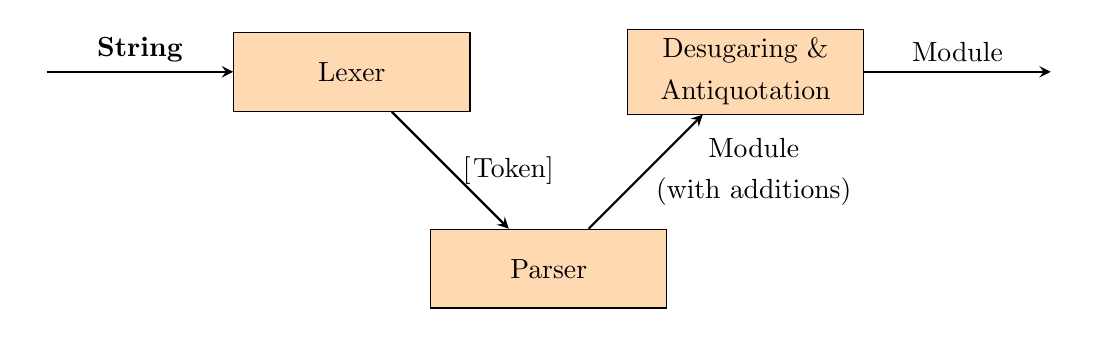
\begin{tikzpicture}[node distance=2.5cm]
\node (start) [draw=none, fill=none] {};
\node (lexer) [process, right of=start, xshift=1.5cm] {Lexer};
\node (parser) [process, below of=lexer, xshift=2.5cm] {Parser};
\node (trans) [process, above of=parser, xshift=2.5cm, align=center] {Desugaring \& \\  Antiquotation};
\node (res) [draw=none, fill=none, right of=trans, xshift=1.5cm] {};

\draw [arrow] (start) -- node[anchor=south] {\lstinline[language=haskell]!String!} (lexer);
\draw [arrow] (lexer) -- node[anchor=west] {\lstinline[language=haskell]![Token]!} (parser);
\draw [arrow] (parser) -- node[anchor=west, align=center] {\lstinline[language=haskell]!Module!\\(with additions)} (trans);
\draw [arrow] (trans) -- node[anchor=south] {\lstinline[language=haskell]!Module!} (res);
\end{tikzpicture}
\end{center}
\caption{flowchart quasiquoter}
\label{fig:quasichart}
\end{figure}

The design of \citetitle{holtz2014quote}, the quasiquoter I defined for LLVM, is inspired by \citetitle{mainland2007c}, which is also used in the cuda implementation of Accelerate.
This means I use \citetitle{alex} to specify the lexer and \citetitle{gill1995happy} for the parser.
The goal of this quasiquoter is to generate an AST as defined by llvm-general-pure.
If I want to do more than just parse complete LLVM code, I can't use this as a target for the parser.
This means it is necessary to copy almost the whole AST and add additional constructors for antiquotation etc.
This step wasn't necessary in \citetitle{mainland2007c} since it's target datastructure still has constructors for antiquotation.

At this point the construction of the 2 quasiquoters differs significantly.
\citetitle{mainland2007c} assumes that constructors stay the same, as long as there isn't a different case available.
It does this by using the function
\begin{lstlisting}[language=haskell]
dataToExpQ :: Data a => (forall b. Data b => b -> Maybe (Q Exp)) -> a -> Q Exp
\end{lstlisting}
This functions converts anything that is of typeclass \lstinline[language=haskell]!Data! into a Template Haskell expression.
In addition to this however, it also takes an extra function to handle exceptions.
This gets executed on every subterm recursively.
If it returns \lstinline[language=haskell]!Nothing!, then the term gets translated into an expression directly.
It it returns \lstinline[language=haskell]!Just exp!, then \lstinline[language=haskell]!exp! is used instead.
The transformation function is then glued together as
\begin{lstlisting}[language=haskell]
qqExp :: Typeable a => a -> Maybe (Q Exp)
qqExp = const Nothing  `extQ` qqStringE
                       `extQ` qqIdE
...
\end{lstlisting}
Since I didn't use the same datatype for input and output, I took a different approach.
I created the following typeclass.
\begin{lstlisting}[language=haskell]
type Conversion a b = forall m.(CodeGenMonad m) => a -> Q (TExp (m b))

class QQExp a b where
  qqExpM :: Conversion a b
  qqExp :: a -> TExpQ b
  qqExp x =
    [||let s = ((0,M.empty) :: (Int,M.Map L.Name [L.Operand])))
       in fst runState $$(qqExpM x) s||]
\end{lstlisting}
The \lstinline[language=haskell]!CodegenMonad! is important mostly to supply new names to unnamed basic blocks.
It also provides an iterface to antiquote a list of basicblocks produced by monadic code generation.
This is necessary to interface with existing code in accelerate-llvm.
\begin{lstlisting}[language=haskell]
class (Applicative m, Monad m) => CodeGenMonad m where
  newVariable    :: m L.Name
  exec           :: m () -> m [L.BasicBlock]
\end{lstlisting}
The \lstinline[language=haskell]!Applicative! context is not necessary since \lstinline[language=haskell]!Monad! is strictly more powerful than \lstinline[language=haskell]!Applicative!.\footnote{With GHC 7.10, \lstinline[language=haskell]!Applicative! will become a superclass of \lstinline[language=haskell]!Monad!.
In the meantime, all instances of \lstinline[language=haskell]!Monad! should be adapted to also provide an instance of \lstinline[language=haskell]!Applicative!.
Details can be found at \url{http://www.haskell.org/haskellwiki/Functor-Applicative-Monad_Proposal}.}
I decided to include it however since it allows for a more concise syntax im my Implementation.

Using a typeclass for the conversion instead of a single function linke in language-c-quote has multiple advantages.
When there is a case missing, it will complain when the quoter is compiled instead of when it is used.
To implement this approach however, the resulting expressions have to be properly typed.
This was not possible before GHC 7.8.

Here is a simple example of an instance declaration of \lstinline[language=haskell]!QQExp!.
\begin{lstlisting}[language=haskell]
instance QQExp A.Module L.Module where
  qqExpM (A.Module n dl tt ds) =
    [||L.Module <$> $$(qqExpM n) <*> $$(qqExpM dl)
                <*> $$(qqExpM tt) <*> $$(qqExpM ds)||]
\end{lstlisting}
In this case the structure of both the source and target constructors are the same.\footnote{Instances like this could be generated using a Template Haskell function.
I decided against using Template Haskell to generate the functions here, since this would make the code harder to debug.}
Antiquotations have to be handled a little different.
Since there can't be any information on the antiquoted expression, it has no specific type.
To use it in a typed expression anyway, it has to be coerced.
\begin{lstlisting}[language=haskell]
instance QQExp A.Operand L.Operand where
  qqExpM (A.AntiOperand s) =
    [||$$(unsafeTExpCoerce $ antiVarE s)||]
\end{lstlisting}
The typed expression is first produced and then splice it into a quoted expression.
This is mostly a cosmetic choice, as the same code could be produced without doing this round trip.

In some cases antiquotation is still a bit cumbersome.
One of these cases is the use of numerical constants.
To antiquote those, it would be necessary to first construct a \lstinline[language=haskell]!Constant!.
I decided it would be nicer if it was also possible to use orfunary Haskell values like \lstinline[language=haskell]!Word32! and \lstinline[language=haskell]!Float! directly.
To this end, I created a class
\begin{lstlisting}[language=haskell]
class ToConstant a where
  toConstant :: a -> L.Constant
\end{lstlisting}
With this it is possible to just write the following:
\begin{lstlisting}[language=haskell]
foo :: Instruction
foo = let i = 5::Word32
      in [lli|add i32 %x, $const:i|]
\end{lstlisting}

\section{Control Structures}
When implementing the control structures, I had to decide on what level I wanted to introduce them.
In a traditional procedural language like C, they would sit alongside the other expressions like assignments or function calls.
This would correspond to the instructions in LLVM.
For this to be possible however, I need to be able to extend them into just a sequence of instructions.
In case of an if-then-else this would kind of be possible using select to get the result value.
This is not the intended way however as side effects are still executed.
Loop structures are an even begger problem, as the number of iterations can be arbitrary.

\subsection{direct approach}
The solution is to have the control structures on the level of basic blocks.
This way it is possible to just produce multiple basic blocks.
For something to behave like a basic block, it must have all the elements of a basic block.
In llvm-general, a basic block is represented as

\begin{lstlisting}[language=haskell]
data BasicBlock =
  BasicBlock Name [Named Instruction] (Named Terminator)
\end{lstlisting}

It consists of a name, a list of instructions and a terminator.
The name is used as a target label for jumps.
The terminator can either be a jump to a different block or a return statement.
The instructions are just a stream without any jumps, but can also contain function calls.

Lets look at a classic for loop.
It starts by initializing a counter.
Then the counter is checked against a maximum.
If this is not yet reached, the loop body gets executed and the counter incremented.
If it is, then the loop exits and the next expression is evaluated.
Figure \ref{fig:forchart} shows the process.

\begin{figure}
\begin{center}
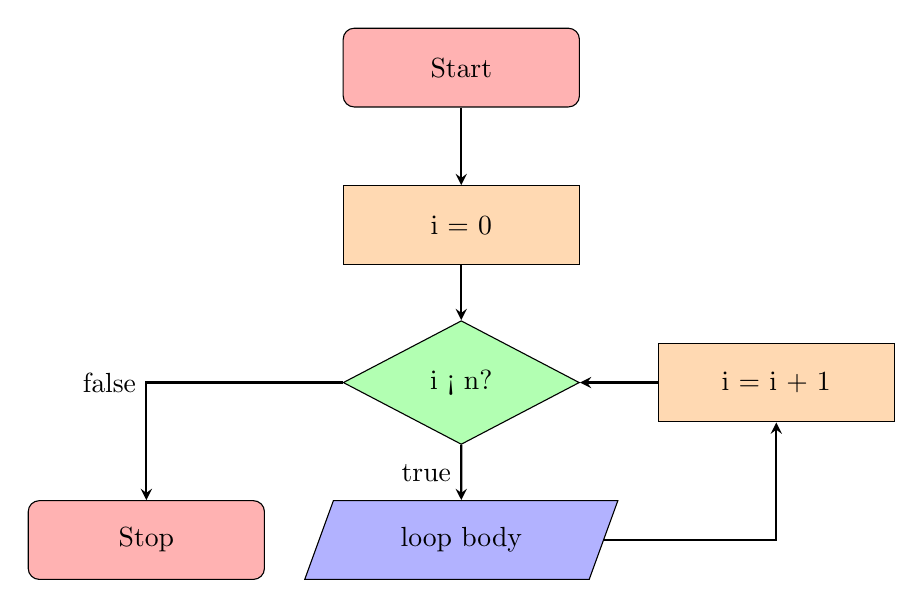
\begin{tikzpicture}[node distance=2cm]
\node (start) [startstop] {Start};
\node (init) [process, below of=start] {i = 0};
\node (check) [decision, below of=init] {i < n?};
\node (body) [io, below of=check] {loop body};
\node (inc) [process, right of=check, xshift=2cm] {i = i + 1};
\node (stop) [startstop, left of=body, xshift=-2cm] {Stop};

\draw [arrow] (start) -- (init);
\draw [arrow] (init) -- (check);
\draw [arrow] (check) --node[anchor=east] {true} (body);
\draw [arrow] (check) -| node[anchor=east] {false} (stop);
\draw [arrow] (body) -| (inc);
\draw [arrow] (inc) -- (check);
\end{tikzpicture}
\end{center}
\caption{flowchart for-loop}
\label{fig:forchart}
\end{figure}

To translate this into LLVM, I need a label, the name of the counter, it's minimum and maximum value and the loop body.
In a normal language these would be sufficient.
LLVM doesn't have mutable variables, however.
This means that any state, like an accumulator, needs to be explicitly defined.
The syntax I chose for this is the following:

\begin{lstlisting}[numbers=none]
for <ty1> <var1> in <val1> to <val2> with <ty2> <values> as <var2>,
           label <jumptarget> { <loop body> }
\end{lstlisting}

The values here work the same way as with \lstinline!phi!-instructions.
It is often necessary to nest loops.
To allow for this, the loop body can consist of multiple basic blocks.
This way, it works much like a function body, with the loop counter and the accumulator as arguments.
Going further with this analogy, I reuse the return statement to indicate the end of the loop.
The value returned is used as the new value of the accumulator.

A simple function summing up the values from \lstinline{%m} to \lstinline{%n-1} would look like the following.
\begin{lstlisting}
i32 foo(i32 %m, i32 %n) {
  entry:
    br label %for

  for:
    for i32 %i in %m to %n with i32 [ 0, %entry ] as %j, label %end {
        %k = add i32 %i, %j
        ret i32 %k
    }

  end:
    ret i32 %j
}
\end{lstlisting}

When implementing this, there are a few things that make matters non-trivial.
Since LLVM doesn't have a concept of mutable variables, it is necessary to introduce \lstinline{phi} instructions manually.
The values that are modified are the accumulator and the loop counter (\lstinline!%j! and \lstinline!%i! in this example).
Each \lstinline{phi} instruction needs one value for each incoming block.
The incoming blocks can be deduced by combining the existing list of incoming values with the return values of block within the loop.
This naturally gives a complete list for the accumulator value.
An additional \lstinline{phi} instruction is then inserted to handle the loop counter.

This is relatively straight forward if you were to implement it as a regular Haskell function.
Working with quasiquoters though, It all has to be implemented in a Template Haskell.
This means that it is sometimes necessary to move code around just so that it compiles, although the types are correct.
The reason for this is the stage restriction of Template Haskell.
A value cannot be spliced into an expression if it was defined locally.
Another big difference is type safety.
Before GHC 7.8, the expressions inside a quoted block would not be typechecked.
You would still get type errors for the code.
Rather than complaining at the definition site it would complain at the usage site however.
This makes defining complex functions nearly impossible.
But even with GHC 7.8 you get some warnings when splicing code in rather than at it's definition site.
For example, it is not checked if a pattern match is exhaustive.
Although this check could be done in the type checker, it is done while desugaring to core.
I filed this as a bug in GHC (\#9113) and it seems that there is work done which would solve this issue.

\subsection{nextblock}
In principle basic blocks are not ordered.
The only exception is the first block, which also cannot have any predecessors.
In reality however, they are mostly ordered in the order of control flow.
With this, it is not strictly necessary to specify which block will be next after a loop as it is mostly the textually next one.
This simplifies the syntax somewhat.

\begin{lstlisting}[numbers=none]
for <ty1> <var1> in <val1> to <val2> with <ty2> <values> as <var2>
           { <loop body> }
\end{lstlisting}

An example of this can be found in figure \ref{fig:forquote}, page \pageref{fig:forquote}.
\todo{write about desugaring}

\begin{itemize}
\item cumbersome syntax
\item limited functionality
\item jumpnext
\end{itemize}

\subsection{antiquotation}
I have so far ignored how antiquotation is handled.
When antiquoting a value, it is usually inserted directly into the AST.
This is straight forward for things like types, constants and operands.
It would be useful however to also antiquote sequences of code.

The existing code in accelerate-llvm uses the \lstinline[language=haskell]!CodeGen! monad to produce code.
\begin{lstlisting}[language=haskell]
data CodeGenState = CodeGenState
  { blockChain          :: Seq Block                            -- blocks for this function
  , symbolTable         :: Map Name AST.Global                  -- global (external) function declarations
  , metadataTable       :: HashMap String (Seq [Maybe Operand]) -- module metadata to be collected
  , intrinsicTable      :: HashMap String Name                  -- standard math intrinsic functions
  , next                :: {-# UNPACK #-} !Word                 -- a name supply
  }
  deriving Show

data Block = Block
  { blockLabel          :: Name                         -- block label
  , instructions        :: Seq (Named Instruction)      -- stack of instructions
  , terminator          :: Maybe (Named Terminator)     -- block terminator
  }
  deriving Show

newtype CodeGen a = CodeGen { runCodeGen :: State CodeGenState a }
  deriving (Functor, Applicative, Monad, MonadState CodeGenState)
\end{lstlisting}

This monad collects instructions into unfinished blocks.
When all blocks are finished, it is then possible to convert these into a list of \lstinline[language=haskell]!BasicBlock!s.
The interesting return values are of type \lstinline[language=haskell]!Operand! or \lstinline[language=haskell]![Operand]!.
To use these in further calculations, they have to be linked to a known value.
This could be achieved by a function
\begin{lstlisting}[language=haskell]
(.=.) :: Operand -> CodeGen Operand -> CodeGen BasicBlock
\end{lstlisting}
The first argument has to be a \lstinline[language=haskell]!LocalReference!.
There is no way to directly assign a value to a name in LLVM without using an additional instruction.
It is however possible to abuse instructions to do exactly this.
The \lstinline!select! instruction can be used in this case.
To do this, both branches of the select have to point to the same value.
This way the additional instruction can be easily removed via constant propagation.

\todo{example}


\subsection{mutable variables}
Although the above methods work, there are some fundamental problems with them.
The fact that you have to specify the variables in the loop header and then return the new value is awkward.
It abuses the return for something that it is not, namely jumping to the loop header.
I could have chosen to use a jump instead, but then there would be no way to update the accumulator.
Another more important flaw is the limitation to one value.
It is possible, of course, to bundle all needed values together in a struct, but this adds a lot of necessary boilerplate code.

In an ordinary language a for loop would consist of just the loop counter and would handle accumulators through mutable variables.
LLVM doesn't support mutable variables however.
Since I need however, I implemented support for them through my quasiquoter.
The implementation is described in \ref{sec:ssa}.

With this idea, the syntax for the for loop is now reduced to
\begin{lstlisting}[numbers=none]
for <ty1> <var1> in <val1> to <val2> { <loop body> }
\end{lstlisting}
This is a great improvement upon the first approach.
The main benefit now is the increased flexibility.
It is also more concise and doesn't abuse the return to pass through variables.

As a side effect, the implementation got a lot simpler.
It is now no longer necessary to scan for return statements to fill \lstinline!phi!-instructions for both counter and accumulator.
Instead, the last block in the loop body just jumps to an end-block, where the counter gets increased and then jumps to the head.
Now the for-loop can be implemented exactly like shown in figure \ref{fig:forchart}.

To allow mutable variables, there has to be a way to initialize them.
The syntax for this is
\begin{lstlisting}[numbers=none]
 <var> = <ty> <val>
\end{lstlisting}
To implement this, I used the select statement.
The above code gets translated into
\begin{lstlisting}[numbers=none]
 <var> = select i1 true, <ty> <val>, <ty> <val>
\end{lstlisting}
It always selects the first value.
Another way would be to leave the second value undefined.
\begin{lstlisting}[numbers=none]
 <var> = select i1 true, <ty> <val>, <ty> undef
\end{lstlisting}
Obviously this adds another unnecessary instruction to the produced code.
This is negligible however, as it is easily removed by LLVM's constant propagation.

\section{SSA}
\label{sec:ssa}
The standard method of producing SSA form in LLVM is to use stack allocated variables instead of registers to store values.
The LLVM optimizer then uses the mem2reg pass to transform these into registers, adding the necessary phi-nodes in the process.

Since one of the goals of the quasiquoter was to produce llvm-code that is as close to what the programmer wrote as possible, I decided against this approach.
Instead I do the transformation myself.
To this end, I provide a single function

\begin{lstlisting}[language=haskell]
toSSA :: [BasicBlock] -> [BasicBlock]
\end{lstlisting}

This is called with the list of all \lstinline[language=haskell]!BasicBlock!'s of a given function.

To produce SSA form, variables have to be versioned, so that it is clear which value it holds at each given time.
There are a multitude of algorithms to do this.
The one most widely used (including in LLVM) is \citeauthor{cytron91efficiently}'s algorithm.
It is however is rather involved as it relies on dominance frontiers.
An easier approach was presented by \citeauthor{braun13simple}.

In this algorithm, the SSA is produced directly from the AST, without the need of extra analysis passes.
To do this, the definitions of variables are tracked and updated as necessary.
Without $\Phi$nodes, this is straight forward, as Figure \ref{fig:localnum} shows.

\begin{figure}
\begin{lstlisting}[language=ruby]
writeVariable(variable, block, value):
    currentDef[variable][block] <- value

readVariable(variable, block):
    if currentDef[variable] contains block:
        # local value numbering
        return currentDef[variable][block]
    # global value numbering
    return readVariableRecursive(variable, block)
\end{lstlisting}
\caption{Implementation of local value numbering}
\label{fig:localnum}
\end{figure}

If the given variable has no definition in the current block, an empty $\Phi$-node is inserted and the local definition is set to the $\Phi$-node.
Now the lookup is done recursively and the values are added to the $\Phi$-node.
This extra step is necessary to detect loops correctly.
I use a slightly different approach than presented in the paper.
The original version tracks if the predecessors of a block are all processed.
This is necessary since only then can the empty $\Phi$-nodes be filled.
This approach makes sense if this is the norm.
In case the input is an unordered list of blocks however, I can't make predictions about this.
Instead I assume that no block is processed until all blocks are.
Figure \ref{fig:globalnum} shows the modified \lstinline[language=haskell]!readVariableRecursive!.

\begin{figure}
\begin{lstlisting}[language=ruby]
readVariableRecursive(variable, block):
    if |block.preds| = 0:
        # First block
        val <- variable
    else:
        # Break potential cycles with operandless phi
        val <- new Phi(block)
        writeVariable(variable, block, val)
    writeVariable(variable, block, val)
    return val
\end{lstlisting}
\caption{Implementation of global value numbering}
\label{fig:globalnum}
\end{figure}

Like most efficient graph algorithms, this algorithm relies heavily on mutable data structures.
Although Haskell - being purely functional - doesn't support these normally, there are multiple methods to implement them inside a pure Monad.
The obvious choices are \lstinline[language=haskell]!State! and \lstinline[language=haskell]!ST!.
\lstinline[language=haskell]!IO! also provides mutable state, but is not an option here, since there is no safe way of running it in a pure context.
I use \lstinline[language=haskell]!ST!, since it natively provides an arbitrary number of mutable variables with direct access.

To use this however, the \lstinline[language=haskell]!BasicBlock!s have to be in a mutable format.

\begin{lstlisting}[language=haskell]
type CFG s =[(Name, MutableBlock s)]

data MutableBlock s = MutableBlock {
  blockName :: Name,
  blockIncompletePhis :: STRef s (M.Map Name (MutableInstruction s)),
  blockPhis :: STRef s [MutableInstruction s],
  blockInstructions :: [MutableInstruction s],
  blockTerminator :: MutableTerminator s,
  blockPreds :: [Name],
  blockDefs :: STRef s (M.Map Name Name)
  }

type MutableInstruction s = STRef s (Named Instruction)
type MutableTerminator  s = STRef s (Named Terminator)
\end{lstlisting}

Although not everything is mutable in this representation, it is sufficient.
After the conversion, the \lstinline[language=haskell]!BasicBlock!s can be processed one by one.
First, the variables created by \lstinline[language=haskell]!Instruction!s are adjusted.
The same is done for usages.
If there a variable is not defined in a given block and there are predecessors, an incomplete \lstinline[language=haskell]!Phi! instruction is added.
Incomplete here means, that the values for every given predecessor are left undefined.
When this is done, the variables referenced by existing \lstinline[language=haskell]!Phi! instructions are replaced by the new values.

Every time a recursive read is done, a new incomplete \lstinline[language=haskell]!Phi! instruction is added.
These are handled last by reading the variable in all preceding blocks and replacing the undefined values.
Since this involved reading however, new incomplete \lstinline[language=haskell]!Phi! instructions can be added in the process.
To handle all of them, the function is executed until there are no incomplete \lstinline[language=haskell]!Phi! instructions.

Figure \ref{fig:tossa} shows the complete \lstinline[language=haskell]!toSSA! function.

\begin{figure}
\begin{lstlisting}[language=haskell]
toSSA :: [BasicBlock] -> [BasicBlock]
toSSA bbs = runST $ do
  cfg <- toCFG $ bbs
  ctr <- newSTRef 1

  -- process all Instructions
  mapM_ (blockToSSAPre ctr) (map snd cfg)
  -- replace names in Phis with correct references
  mapM_ (blockToSSAPhi ctr cfg) (map snd cfg)
  -- replace names in newly added Phis with correct references
  handleIncompletePhis ctr cfg

  fromCFG cfg
\end{lstlisting}
\caption{\lstinline[language=haskell]!toSSA!}
\label{fig:tossa}
\end{figure}

\chapter{Skeletons}
The skeletons are one of the core components of an accelerate backend.
They provide the functionality of a given array function like \lstinline[language=haskell]!map! or \lstinline[language=haskell]!fold!.
They are basically functions that given extra arguments for array environment and higher order function generate a concrete function which can then be compiled.
In accelerate-llvm, this process is abstracted through a typeclass.
\begin{lstlisting}[language=haskell]
class Skeleton arch where
  generate      :: (Shape sh, Elt e)
                => arch
                -> Gamma aenv
                -> IRFun1 aenv (sh -> e)
                -> CodeGen [Kernel arch aenv (Array sh e)]
  ...
\end{lstlisting}
Each of the different functions in this class corresponds to a specific skeleton.

When implementing parallel algorithms, it often becomes more complicated.
Accelerate was specifically designed to only consist of operations that can be implemented efficiently.

In the following, I will go through the skeletons one by one.
\section{generate}
The simplest skeleton is \lstinline[language=haskell]!generate!.
As the name suggests, it produces an array with just a function from index to a value.
\begin{lstlisting}[language=haskell]
mkGenerate
    :: forall arch aenv sh e. (Shape sh, Elt e)
    => Gamma aenv
    -> IRFun1 aenv (sh -> e)
    -> CodeGen [Kernel arch aenv (Array sh e)]
\end{lstlisting}
Before the actual quasiquoted llvm code, we have to set up some values first.
The first thing we need are the parameters for the output array and the array environment.
The start and stop indices are also required.
\begin{lstlisting}[language=haskell]
mkGenerate aenv apply =
  let
      arrOut   = arrayDataOp  (undefined::Array sh e) "out"
      shOut    = arrayShapeOp (undefined::Array sh e) "out"
      paramOut = arrayParam   (undefined::Array sh e) "out"
      paramEnv = envParam aenv
      (start, end, paramGang)
               = gangParam
\end{lstlisting}
The last piece before the actual code are some declarations for used types and local variables.
\begin{lstlisting}[language=haskell]
      intType  = typeOf (int :: IntegralType Int)

      r        = locals (undefined::e) "r"
      i        = local intType "i"
      ix       = locals (undefined::sh) "ix"
\end{lstlisting}
The rest is then relatively self-explaining.
\begin{lstlisting}
  in
  makeKernelQ "generate" [llgM|
    define void @generate
    (
        $params:paramGang,
        $params:paramOut,
        $params:paramEnv
    )
    {
        for $type:intType %i in $opr:start to $opr:end
        {
            ;; convert to multidimensional index
            $bbsM:(ix .=. indexOfInt shOut i)
            ;; apply generator function
            $bbsM:(r  .=. apply ix)
            ;; store result
            $bbsM:(writeArray arrOut i r)
        }
        ret void
    }
  |]
\end{lstlisting}
\subsection{vectorization}
If \lstinline[language=haskell]!generate! vectorizes is very dependent on the supplied function.
A function which randomly references a different manifest array would not vectorize for example.
The challinging part for the optimizer are the multidimensional indices.
This means the chance of vectorization is much higher if the target is just a vector.

\section{map}
\lstinline[language=haskell]!map! works similar to \lstinline[language=haskell]!generate!.
In fact it can be easily implemented using \lstinline[language=haskell]!generate!.
One important difference between \lstinline[language=haskell]!generate! and \lstinline[language=haskell]!map! is how they access the array.
\lstinline[language=haskell]!generate! works with multidimensional indices.
This is not necessary with \lstinline[language=haskell]!map! however, as \lstinline[language=haskell]!map! keeps indices identical.

\begin{lstlisting}[language=haskell]
mkMap :: forall t aenv sh a b. (Elt b, Elt a)
      => Gamma aenv
      -> IRFun1    aenv (a -> b)
      -> IRDelayed aenv (Array sh a)
      -> CodeGen [Kernel t aenv (Array sh b)]
\end{lstlisting}
The following is the core part of the \lstinline[language=haskell]!map! skeleton.
I omit the rest of the function as the difference to \lstinline[language=haskell]!generate! is mostly mechanical.
\begin{lstlisting}
makeKernelQ "map" [llgM|
    define void @map
    (
        $params:paramGang,
        $params:paramOut,
        $params:paramEnv
    )
    {
        for $type:intType %i in $opr:start to $opr:end
        {
            $bbsM:(x .=. delayedLinearIndex [i])
            $bbsM:(y .=. apply x)
            $bbsM:(writeArray arrOut i y)
        }
        ret void
    }
  |]
\end{lstlisting}

\subsection{vectorization}
\lstinline[language=haskell]!map! vectorizes far better than \lstinline[language=haskell]!generate!.
If the supplied array is manifest, no index conversion is necessary.
If the function doesn't contain branches, then it is very likely that vectorization is possible.

\section{transform}
\lstinline[language=haskell]!transform! is closely related to map.
The difference is, that the index is not preserved.
Instead there is another function which projects an index in the target array into an index in the source array.
\begin{lstlisting}[language=haskell]
defaultTransform
    :: (Shape sh, Shape sh', Elt a, Elt b, Skeleton arch)
    => arch
    -> Gamma aenv
    -> IRFun1    aenv (sh' -> sh)
    -> IRFun1    aenv (a -> b)
    -> IRDelayed aenv (Array sh a)
    -> CodeGen [Kernel arch aenv (Array sh' b)]
\end{lstlisting}
In fact \lstinline[language=haskell]!map! can be easily implemented using transform:
\begin{lstlisting}[language=haskell]
defaultMap arch aenv f a = transform arch aenv return f a
\end{lstlisting}
We keep a seperate implementation of \lstinline[language=haskell]!map! however for performance reasons.
The specific reason for this is that \lstinline[language=haskell]!map! preserves the the indices.
Since \lstinline[language=haskell]!transform! doesn't have this property, we simply implement it in terms of \lstinline[language=haskell]!generate!.
\begin{lstlisting}[language=haskell]
defaultTransform arch aenv p f IRDelayed{..} =
  generate arch aenv $ \ix -> do
    ix' <- p ix
    a   <- delayedIndex ix'
    f a
\end{lstlisting}

\subsection{vectorization}
If \lstinline[language=haskell]!transform! vectorizes is very dependent on the functions involved.
In case of a simple identity (\lstinline[language=haskell]!map!) it will vectorize just fine.
It is however really not at all guaranteed, that it will vectorize.
A simple counter example is the following.
\begin{lstlisting}[language=haskell]
let a0 = use (Array (Z :. 10) [1,2,3,4,5,6,7,8,9,10])
in backpermute (Z :. 10) (\x0 -> Z :. mod (1 + (indexHead x0),indexHead (shape a0))) a0
\end{lstlisting}
All this code does is rotate the array to the right by one element and then adding one.
This code, if optimized by hand, could be easily vectorized.

To give another positive example, let's look at the reversal of an array.
\begin{lstlisting}[language=haskell]
let a0 = use (Array (Z :. 10) [1,2,3,4,5,6,7,8,9,10])
in transform
     (shape a0) (\x0 -> Z :. -1 + ((indexHead (shape a0)) - (indexHead x0))) (\x0 -> 1 + x0) a0
\end{lstlisting}
This vectorizes just fine.
LLVM uses \lstinline{shufflevector} to achieve this.
\begin{lstlisting}
...
%reverse = shufflevector <4 x i64> %wide.load, <4 x i64> undef, <4 x i32> <i32 3, i32 2, i32 1, i32 0>
...
\end{lstlisting}

\subsection{backpermute}
Accelerate handles a special case of \lstinline[language=haskell]!transform! as \lstinline[language=haskell]!backpermute!.
This is essentially just a transform without the map functionality.
We don't have a specific implementation of \lstinline[language=haskell]!backpermute!, but rather use \lstinline[language=haskell]!transform!.
\begin{lstlisting}[language=haskell]
defaultBackpermute
    :: (Shape sh, Shape sh', Elt e, Skeleton arch)
    => arch
    -> Gamma aenv
    -> IRFun1    aenv (sh' -> sh)
    -> IRDelayed aenv (Array sh e)
    -> CodeGen [Kernel arch aenv (Array sh' e)]
defaultBackpermute arch aenv p a = transform arch aenv p return a
\end{lstlisting}

\section{permute}
\lstinline[language=haskell]!permute! is analog to \lstinline[language=haskell]!backpermute!.
Instead of projecting every cell of the target array onto a cell in the source array, the opposite is done.
Every cell in the source array is projected onto one or no cell in the target array.
There is no assumption being made about this projection.
This means there can be either multiple or no cell pointing to a single output cell.
To deal with no projection the output array is initialized with a given array.
To deal with multiple cells, there is a function to combine the existing value with the new one.
\begin{lstlisting}[language=haskell]
mkPermute
    :: forall arch aenv sh sh' e. (Shape sh, Shape sh', Elt e)
    => Gamma aenv
    -> IRFun2 aenv (e -> e -> e)
    -> IRFun1 aenv (sh -> sh')
    -> IRDelayed aenv (Array sh e)
    -> CodeGen [Kernel arch aenv (Array sh' e)]
\end{lstlisting}

To get the values, the loop goes over all the elements in the source array.
This is then projected into the target array.
\begin{lstlisting}
  makeKernelQ "permute" [llgM||
    define void @permute
    (
        $params:paramGang,
        $params:paramBarrier,
        $params:paramOut,
        $params:paramEnv
    )
    {
        for $type:intType %i in $opr:start to $opr:end
        {
            $bbsM:(ix .=. indexOfInt shOut i)
            $bbsM:(ix' .=. permute ix)
...
            }
        }
        ret void
    }||]
\end{lstlisting}
There is however an option that the index is not projected at all.
This is signalled by a magic value \lstinline[language=haskell]!ignore!.
In this case the inner loop is empty.
\begin{lstlisting}
            ;; If this index will not be used, jump immediately to the exit
            $bbsM:(c1 .=. all (uncurry (neq int)) (zip ix' ignore))
            if %c1 {
...
            }
\end{lstlisting}
If the value is not ignored, the permutation step will be executed.
\begin{lstlisting}
                $bbsM:(old .=. readArray arrOut dst)
                $bbsM:(new .=. delayedLinearIndex [i])
                $bbsM:(val .=. combine new old)
                $bbsM:(writeArray arrOut dst val)
\end{lstlisting}
This would be enough in a single-threaded context.
In a multi-threaded context this is not enough however.
In that case, this central step is a critical section.
This means it has to be executed atomically.
To achieve this, we have a vector of essentially booleans.
This vector has an element for every element of the result array.
We use special atomic memory operation to use these for a spinlock.

First we have to determine the specific memory cell to use.
\begin{lstlisting}
                %baddr = getelementptr i8* $opr:barrier, $type:intType $opr:dst
\end{lstlisting}
With this, we can now look at the the lock is taken.
\begin{lstlisting}
                %c2 = i1 true
                while %c2 {
                    %lock = atomicrmw volatile xchg i8* %baddr, i8 1 acq_rel
                    %c2 = icmp eq i8 %lock, 0
                }
\end{lstlisting}
\lstinline!atomicrmw volatile xchg! excanges the current value with a new value and returns the old one.
This way we know if the lock was taken before or not.
\lstinline!volatile! signals that the operations can't be reordered.
This pattern is common enough, that modern CPUs have optimizations in place.
The associated cache line will be shared between all CPUs/cores.
This was there is no unnecessary bus traffic.

The lock release is less involved.
\begin{lstinline}
                store atomic volatile i8 0, i8* %baddr release, align 1
\end{lstinline}
It is possible to use a regular store here.
This will be translated into just a MOV instruction.
This is possible due to subtle memory ordering rules which allow this, even though MOV is not a full memory barrier.
In case of other architectures like ARM a MOV is not sufficient here.

\subsection{vectorization}
Vectorization is not possible in case of \lstinline[language=haskell]!permute!.
In every step, the same cell in the output array is both read and written.
The only way this could possibly vectorize is if this index was predictable.

That said, the current implementation cannot possibly vectorize.
What blocks the vectorization is the synchronization via spinlocks.
It may be beneficial to supply an additional implementation for single-threaded execution.
This would not need the extra array of semaphores.
I leave this evaluation for future work.

\section{fold}
In Haskell, a fold reduces a list to a single value.
The equivalent would be to reduce a vector to a scalar.
While Accelerate also supports this, it has a more general view.
It is possible to also reduce an Array of arbitrary dimensionality.
The result will then be an array with it's inner dimension reduced.

\begin{lstlisting}[language=haskell]
mkFold
    :: forall t aenv sh e. (Shape sh, Elt e)
    => Gamma aenv
    -> IRFun2    aenv (e -> e -> e)
    -> IRExp     aenv e
    -> IRDelayed aenv (Array (sh:.Int) e)
    -> CodeGen [Kernel t aenv (Array sh e)]
\end{lstlisting}

The natural unit of computation for a fold is one element in the output array.
This degree of parallelism can be achieved without multiple passes.
\begin{lstlisting}
  makeKernelQ "fold" [llgM|
    define void @fold
    (
        $params:paramGang,
        $params:paramStride,
        $params:paramOut,
        $params:paramEnv
    )
    {
      %sz = mul $type:intType $opr:start, $opr:n

      for $type:intType %sh in $opr:start to $opr:end
      {
          %next = add $type:intType %sz, $opr:n
          $bbsM:(x .=. seed)

        reduce:
          for $type:intType %i in %sz to %next
          {
              $bbsM:(y .=. delayedLinearIndex [i])
              $bbsM:(x .=. combine x y)
          }

          $bbsM:(writeArray arrOut sh x)
          %sz = $type:intType %next
      }
      ret void
    }
  |]
\end{lstlisting}
This works great if the output still has a dimension left.
If the output is a skalar however, it doesn't work that well.
Instead, the array is reduced in multiple steps.
The first step is to create an array of partial sums.
This array can then be reduced by a single thread sequentially.

\subsection{segmented fold}
The segmented fold is a generalization of the regular fold.
The regular fold reduces the inner dimension to a single value.
The segmented fold reduces segments of the inner dimension into single values.
This way the dimensionality of the resulting array is the same as the incoming array.
The degree of parallelism is increased by the same amount as there are segments.

\subsection{vectorization}
In general, fold doesn't vectorize very well.
\lstinline[language=haskell]!fold! requires it's input function to be associative.
For LLVMs loop vectorization to work however, it also needs to be commutative.
Many associative functions are also commutative however.
This means that these cases will vectorize well.

\section{scan}
Scan (or prefix sum) is closely related to fold.
Instead of just providing one value at the end however, it produces all the values in between.
In contrast to fold, scan only operates on vectors.
This makes implementation somewhat easier, as there is no special case for this as with \lstinline[language=haskell]!foldAll!.
Scan also comes in different flavours: \lstinline[language=haskell]!scanl!, \lstinline[language=haskell]!scanr!, \lstinline[language=haskell]!scanl'! and \lstinline[language=haskell]!scanr'!.
I will focus only on \lstinline[language=haskell]!scanl! here, as the differences are mostly mechanical.

\begin{lstlisting}[language=haskell]
mkScanl
    :: forall t aenv e. (Elt e)
    => Gamma aenv
    -> IRFun2    aenv (e -> e -> e)
    -> IRExp     aenv e
    -> IRDelayed aenv (Vector e)
    -> CodeGen [Kernel t aenv (Vector e)]
\end{lstlisting}

As with \lstinline[language=haskell]!fold!, the implementation of prefix sums differs between non-parallel and parallel.
Scan is difficult to implement as a parallel algorithm.
Every element depends on its direct predecessor.
The approach I took was:

\begin{enumerate}
\item divide the array into chunks
\item build the sum of each chunk
\item build the prefix sums over those sums
\item use the prefix sums as starting point to build the final array
\end{enumerate}

This approach requires 2 read operation and 1 write operation asymptotically.
I decided to build combine the last 2 steps into one.
The last step is done completely in parallel, so this leads to some extra work.
Depending on the size of the array this may be faster as calling into a kernel has some overhead.
I leave this evaluation for future work.

The first 2 steps of the process are basically identical to the multidimensional fold.
The rest forms one big kernels, as I essentially combine 2 separate operations into one.

First look at the function parameters.
\begin{lstlisting}
  makeKernelQ "scanl" [llgM|
    define void @scanl
    (
        $params:paramGang,
        $type:intType %lastChunk,
        $type:intType %chunkSize,
        $type:intType %sz,
        $params:paramTmp,
        $params:paramOut,
        $params:paramEnv
    )
    {
        for $type:intType %i in $opr:start to $opr:end
        {
...
        }
        ret void
    }
  |]
\end{lstlisting}
The gang parameters (start, stop) in this case are measured not in single elements, but in chunks.
The size of these chunks is given by \lstinline{%chunksize}.
The total length and the number of chunks is also provided.
This is necessary to handle the last chunk as it is not of full length.

The first step then is the scan over the previously computed sums.
The seed element is also written to the first array index in this step.
\begin{lstlisting}
            ;; sum up the partial sums to get the first element
            $bbsM:(acc .=. seed)

            for $type:intType %k in 0 to %i
            {
                $bbsM:(x .=. delayedLinearIndex tmpD [k])
                $bbsM:(acc .=. combine x acc)
            }

            ;; check if this is the first chunk
            %c2 = icmp eq $type:intType %i, 0
            ;; if it is, write the seed to memory
            if %c2 {
                %c3 = icmp ne $type:intType %sz, 0
                if %c3 {
                    $bbsM:(writeArray arrOut zero acc)
                }
            }
\end{lstlisting}
The outer loop just gives the chunk number.
This has to be converted into a usable range first.
\begin{lstlisting}
            ;; calculate the start of the current chunk
            %ix    = mul $type:intType %i,  %chunkSize
            ;; Determine the end of the current chunk. If this is the last chunk,
            ;; then this is the same as the end of the array.
            %last1 = add $type:intType %ix, %chunkSize
            %c1    = icmp eq $type:intType %i, %lastChunk
            %last  = select i1 %c1, $type:intType %sz, $type:intType %last1
\end{lstlisting}
With the correct range and the prefixsum of all previous elements, the rest is easy.
\begin{lstlisting}
          reduce:
            for $type:intType %k in %ix to %last
            {
                %k1 = add $type:intType %k, 1
                $bbsM:(x .=. delayedLinearIndex inD [k])
                $bbsM:(acc .=. combine acc x)
                $bbsM:(writeArray arrOut k1 acc)
            }
\end{lstlisting}

I didn't define a seperate function for the sequential case.
It is easy though to use the exact same function as above though.
It is only necessary to supply an empty array of precalculated sums.
This way the scan over that array yields the just seed element.
This is then used to compute the prefix sum directly.

\subsection{vectorization}
The steps equivalent to a fold vectorize very well.
The this is in essence all but the last step.
The actual prefix sum cannot be vectorized, as all the intermediate values have to be written to memory.

\section{stencil}
Stencil operations are basically a generalization of map.
The difference is that the focus is not on a single element.
Instead it also looks at the surrounding cells.

\begin{lstlisting}[language=haskell]
mkStencil
  :: forall arch aenv sh stencil a b. (Elt b, Stencil sh a stencil)
  => Gamma aenv
  -> Proxy (stencil,a)
  -> IRFun1 aenv (stencil -> b)
  -> Boundary (IRExp aenv a)
  -> CodeGen [Kernel arch aenv (Array sh b)]
\end{lstlisting}

This is leads to a problem however.
While \lstinline[language=haskell]!map! is always guaranteed to read in bounds, this can't be said about stencils.
There are multiple ways to avoid this problem.
Accelerate tries to capture the different options via the \lstinline[language=haskell]!Boundary! type.
\begin{lstlisting}[language=haskell]
data Boundary a
  = Clamp       -- ^clamp coordinates to the extent of the array
  | Mirror      -- ^mirror coordinates beyond the array extent
  | Wrap        -- ^wrap coordinates around on each dimension
  | Constant a  -- ^use a constant value for outlying coordinates
\end{lstlisting}
They can be divided into 2 groups.
All except \lstinline[language=haskell]!Constant! rely on index manipulation.
\lstinline[language=haskell]!Constant! on the other hand does no read at all if the read would be out of bounds.
I use a single function \lstinline[language=haskell]!access! to deal with all of these cases.
The returned value is a the value read at the given index modulo the boundary condition.
I start by applying the offset to the index.
If the offset is 0 in every direction however, the read can be done directly.
\begin{lstlisting}[language=haskell]
access bndy sh ix arr off =
  if all (==0) off
    then do
      i <- intOfIndex sh ix
      readArray arr i
    else do
      ix' <- zipWithM (add int . (constOp . num int)) off ix
\end{lstlisting}
This gives me the correct cell to do the read on.
Then I group the Boundary into \lstinline[language=haskell]!Constant! and the rest.
In this step I also replace the boundary with its corresponding handler function.
\begin{lstlisting}[language=haskell]
  let op = case bndy of
        Constant as -> Left as
        Clamp       -> Right clamp
        Mirror      -> Right mirror
        Wrap        -> Right wrap
\end{lstlisting}
Now all is left is to do the boundary checks and the read.
In case of \lstinline[language=haskell]!Clamp!, \lstinline[language=haskell]!Mirror! and \lstinline[language=haskell]!Wrap! this is straight forward.
\begin{lstlisting}[language=haskell]
  case op of
    Right op' -> do
      ix'' <- op' sh ix'
      i <- intOfIndex sh ix''
      readArray arr i
\end{lstlisting}
In case of \lstinline[language=haskell]!Constant! however this is a little more complicated.
\begin{lstlisting}[language=haskell]
    Left as -> do
      as'       <- as
      ix''      <- wrap sh ix'
      i         <- intOfIndex sh ix''
      c         <- inRange sh ix'
      zipWithM (\a x -> instr (typeOfOperand a) (Select c x a [])) as' xs
\end{lstlisting}
I prepare both the constant and the read value.
I then do the bounds check and select either value depending on the result.
To avoid out of bounds reads, I wrap the index before I read it.
This is necessary since it is fairly easy to construct stencil functions that would end in a segfault otherwise.

The complete stencil is then constructed via the function \lstinline[language=haskell]!stencilAccess!.
\begin{lstlisting}[language=haskell]
stencilAccess
  :: forall a b sh aenv stencil. (Shape sh, Stencil sh a stencil)
  => Proxy (stencil,a)
  -> Proxy sh
  -> [Operand]
  -> [Operand]
  -> Boundary (IRExp aenv a)
  -> IRFun1 aenv (sh -> stencil)
stencilAccess _ _ sh arr bndy ix = do
  let off     = offsets (undefined :: Fun aenv (stencil -> a))
                        (undefined :: OpenAcc aenv (Array sh a))
      off'    = map (map (constOp . num int) . reverse . shapeToList) off
  stencil <- mapM (access bndy sh ix arr) off'
  return (concat stencil)
\end{lstlisting}
The \lstinline[language=haskell]!Proxy! values immediately look out of place.
It seems that the types are already present in the \lstinline[language=haskell]!Boundary! and the result type.
They are necessary however, as those are just type synonyms.
Apart from this oddity, there isn't much happening in this function.
It mainly combines existing offsets and applies the \lstinline[language=haskell]!access! function.

All that remains now is the actual skeleton code.
This looks very similar to the \lstinline[language=haskell]!map! skeleton.
\begin{lstlisting}
  makeKernelQ "stencil" [llgM|
    define void @stencil
    (
        $params:paramGang,
        $params:paramIn,
        $params:paramOut,
        $params:paramEnv
    )
    {
        for $type:intType %i in $opr:start to $opr:end
        {
            $bbsM:(ix .=. indexOfInt shOut i)
            $bbsM:(x .=. (stencilAccess stencilT shT shIn arrIn bndy ix >>= apply))
            $bbsM:(writeArray arrOut i x)
        }
        ret void
    }
  |]
\end{lstlisting}
The code for \lstinline[language=haskell]!stencil2! is analogous.

\subsection{vectorization}
The stencil code doesn't vectorize at all at the moment.
The reason for this is the boundary.
If the whole stencil is guaranteed to be in bounds, the bounds check could be omitted however.
This way the read would be guaranteed to vectorize.

\chapter{Results}
\section{Benchmarks}

The Benchmarks were run on a dual CPU Xeon E5-2650 (16 cores, 2GHz, 64GB RAM) running GNU/Linux (Ubuntu 12.04 LTS).
Programs are compiled with ghc-7.8.3 and llvm-3.4.2.
All programs are executed on all 16 cores unless stated otherwise.

\subsection{Ray Tracer}
\begin{figure}
    \centering
    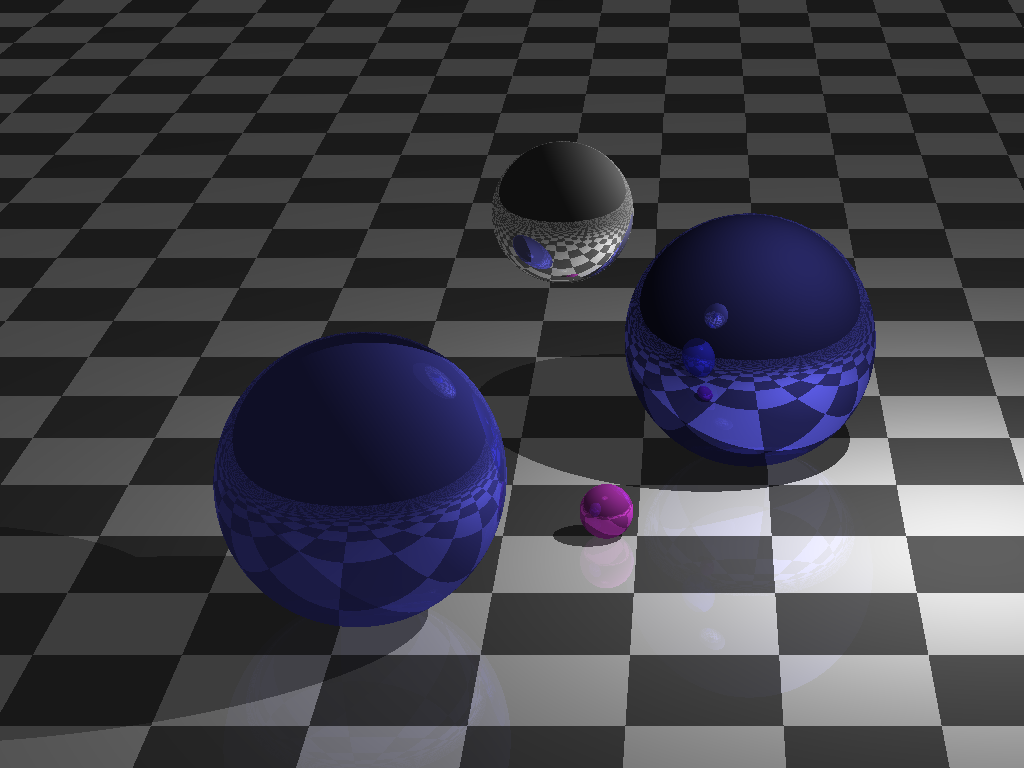
\includegraphics[width=0.8\textwidth]{images/benchmarks/ray/ray_sample}
    \caption[Ray tracer]{Image of a ray traced scene rendered on the GPU with
    Accelerate, featuring multiple reflections. The scene is animated and
    renders in real time on modest hardware.}
    \label{fig:ray_sample}
\end{figure}

Ray tracing is a technique for generating an image by tracing the path of light through pixels in an image plane and simulating the effects of its encounters with virtual objects.
The technique is capable of producing a very high degree of realism compared to typical scanline rendering methods, as ray tracing algorithms are able to simulate optical effects such as reflection and refraction, scattering, and dispersion phenomena.
This increased accuracy has a larger computational cost, which is why ray tracing is not typically used for real time rendering applications such as computer games.
Figure \ref{fig:ray_sample} shows the result of rendering a scene using a ray-tracer implemented in Accelerate.
The algorithm computes the colour of a pixel by casting a ray from that point in a specified direction, and tracing its interaction with the objects in the scene.

After fusion, this ends up being just a single generate kernel.
Figure \ref{fig:ray_bench} shows the runtime of the ray-tracer for different image sizes.
The comparison here is against a Repa implementation of the same algorithm.
Independent of the image size, the Accelerate version is about 45\% faster than the Repa version.
\todo{reasoning}
\begin{figure}
    \centering
    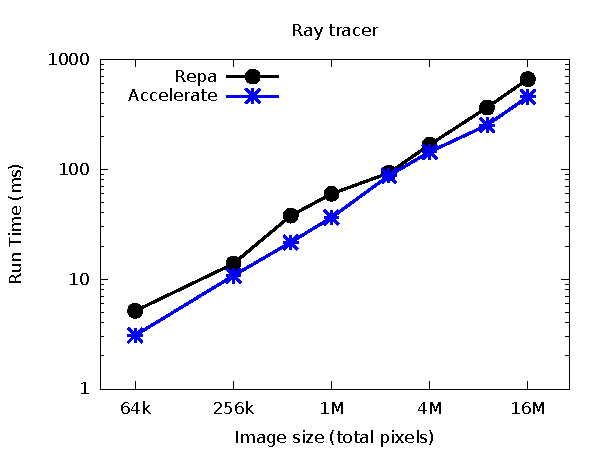
\includegraphics[width=0.8\textwidth]{images/benchmarks/ray/ray}
    \label{fig:ray_bench}
\end{figure}

Accellerate-llvm has very heavy infrastructure in place to synchronize threads.
The intuition is, that this might lead to decreased scalability.
Figure \ref{fig:ray_scale} shows the speedup per core using the raytracer.
As you can see, Accelerate performs basically identical to Repa in this regard.

\begin{figure}
    \centering
    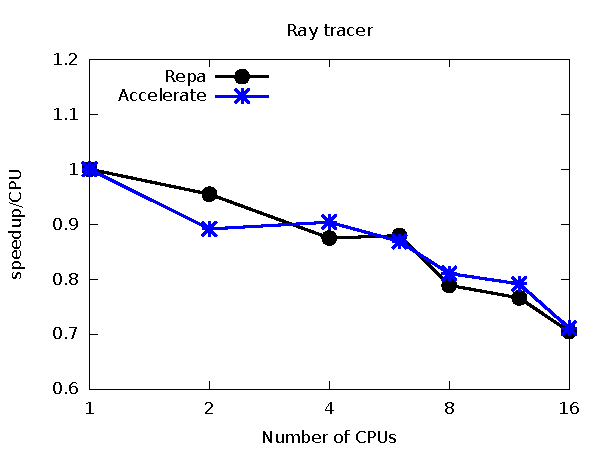
\includegraphics[width=0.8\textwidth]{images/benchmarks/ray/ray-scale}
    \label{fig:ray_scale}
\end{figure}

\subsection{N-Body}
The $n$-body example simulates the Newtonian gravitational forces on a set of massive bodies in 3D space, using the na\"ive $\mathcal{O}\left( n^{2} \right)$ algorithm.
In a data-parallel setting, the natural way to express this algorithm is first to compute the forces between every pair of bodies, before adding the forces applied to each body using a segmented sum.
Figure \ref{fig:nbody} shows the results of this program in different settings.

\begin{figure}
    \centering
    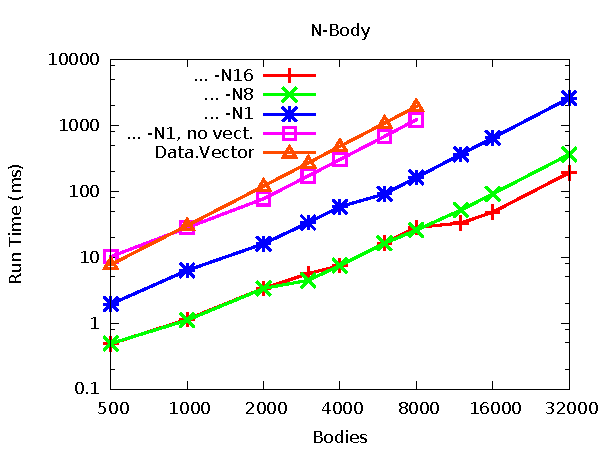
\includegraphics[width=0.8\textwidth]{images/benchmarks/nbody/nbody}
    \label{fig:nbody}
\end{figure}

After fusion, this example consists of a \lstinline[language=haskell]!generate! and a \lstinline[language=haskell]!map! kernel.
Both of these vectorize well.
This is clear when looking at the difference in runtime between the vectorized and unvectorized kernels executed in a single thread.
The difference between them is almost a factor of 8, which is the vector width for floats on the benchmark machine.

Another interesting point here is how it performs against an implementation using \lstinline[language=haskell]!Data.Vector!.
For small sizes, \lstinline[language=haskell]!Data.Vector! is faster than Accelerate.
This is due to the overhead Accelerate brings to the table.
For bigger sizes Accelerate is significantly faster however.

When running with \texttt{+RTS -N16}, it doesn't scale quite as well as the raytracer for smaller sizes.
This is likely due to memory transfers.
The Benchmark machine is a dual CPU server and therefore can't share the on-chip cache between all available cores.
In fact the runtime is identical whether executed with 8 or 16 cores.
On very large datasets (>12000 bodies) this is no longer the case and the extra parallelism is noticeable.

\subsection{Canny Edge Detection}
The Canny edge detector is an edge detection operator that uses a multi-stage algorithm to detect a wide range of edges in images.
It was developed by John F. Canny in 1986.
Canny edge detection is a four step process.
\begin{enumerate}
\item A Gaussian blur is applied to clear any speckles and free the image of noise.
\item A gradient operator is applied for obtaining the gradients' intensity and direction.
\item Non-maximum suppression determines if the pixel is a better candidate for an edge than its neighbours.
\item Hysteresis thresholding finds where edges begin and end.
\end{enumerate}

An example of the algorithm in action is shown in figure \ref{fig:lena}.

\begin{figure}
    \centering
    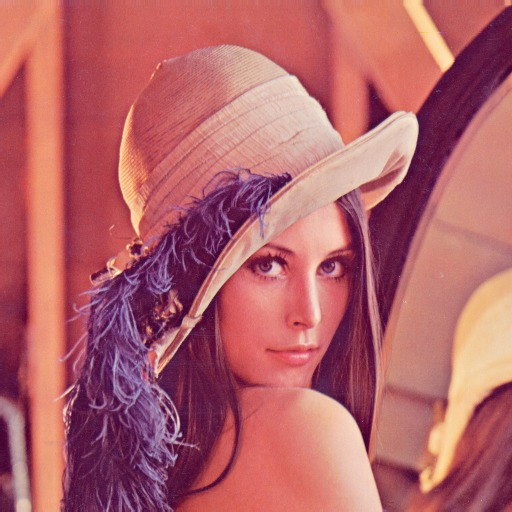
\includegraphics[width=0.4\textwidth]{images/benchmarks/canny/lena}
    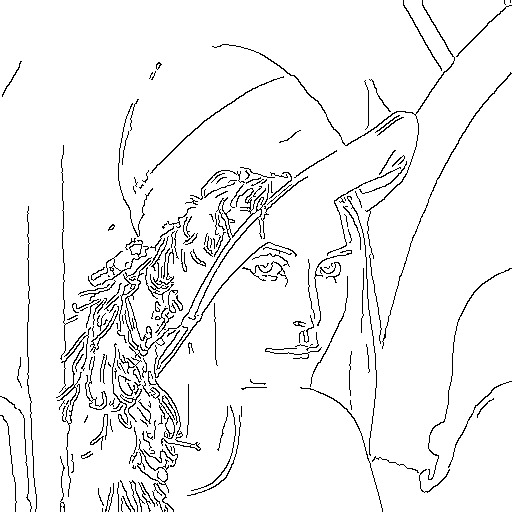
\includegraphics[width=0.4\textwidth]{images/benchmarks/canny/lena-edges}
    \label{fig:lena}
\end{figure}

The Canny Edge Detection consists mainly of stencil convolutions.
These are very specialized operations.
Figure \ref{fig:canny} shows the run time for different image sizes.
The Repa and Accelerate versions both execute on 16 cores while the OpenCV version only uses one CPU.
Accelerate is consistently faster than Repa in this benchmark.
On small image sizes, the OpenCV version, even though only running on 1 core, is significantly faster than both Accelerate and Repa.
With larger image sizes, this difference becomes smaller.
One important difference is, that OpenCV is carefully optimized to vectorize well.
The skeleton code for stencils is barely optimized at all and hence doesn't vectorize.
Repa cannot vectorize for technical reasons.\cite{lippmeier2012efficient}

\begin{figure}
    \centering
    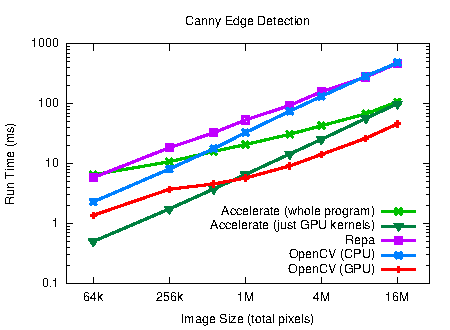
\includegraphics[width=0.8\textwidth]{images/benchmarks/canny/canny}
    \label{fig:canny}
\end{figure}

\chapter{Conclusion}
Prior to this thesis, only a handful of skeletons were implemented in the llvm backend to accelerate.
These worked, but were hard to read as the tool used relied on manipulating blocks directly.
In this thesis I presented an alternative approach to code generation for llvm.
I implemented the remaining skeletons and rewrote the existing ones using my quasiquoter.
The resulting code is much more legible and therefore maintainable than the purely monadic approach taken by previous work.

One reason for using LLVM as the target is, that it is very clear what the produced code will look like on assembler-level.
I was important for me not to compromise this advantage.
I parse LLVM Instructions directly without modification, so it is guaranteed that the user has absolute control over the generated code.
To improve legibility and maintainability, I introduced concepts from high-level languages like mutable variables and control structures.
These are purely an addition to the existing LLVM language and are translated into LLVM code by the quasiquoter.

Using a foreign library in Haskell is often tedious, as the main documentation doesn't quite line up with the Haskell bindings.
LLVM is no exception to this, although the AST used is very well documented.
This where the quasiquoter shines, as the instructions are exactly the same as documented in the language reference.

Most languages model variables as cells in memory.
This is fine, as LLVM is capable to lower these into register values if possible.
The code already present in the LLVM backend didn't use this method however, so the quasiquoter doesn't use this mechanism.
Instead, it treats regular LLVM values as variables that can be re-assigned at any time.
To this end, I implemented a transformation back into legal LLVM code.
The resulting language has everything you would expect from an imperative language like mutable variables and control structures.
In this way, it ``feels'' much like programming in C, while still having a clear representation in LLVM IR.

\section{Related Work}
Haskell offers a range of ways to implement operations on arrays effectively.
The one most closely resembling Accelerate is Repa.
As in the LLVM backend described in this thesis, it uses gang workers to execute computations on multiple CPUs concurrently.
The important difference between Accelerate and Repa is the execution model.
While Repa computations behave like any other Haskell computation, Accelerate behaves more like running a Monad.
Since Accelerate is device-independent, it has to compile the needed functions at runtime before the actual computation can occur.

In terms of code generation, C-- most closely resembles the language I created.
It was designed as an intermediate language for compilers and is in use in GHC.
It's design is inspired by C, but it replaces many language elements for clearer definitions.
Like LLVM, it's type system is deliberately designed to reflect constraints of the underlying hardware.
There is however no clear standard implementation for C--, making it more difficult to use than LLVM.

\section{Future Work}
I developed the quasiquoter mainly as a tool to use for skeleton code generation.
This means, that the main focus was on generating code for complete functions.
It should be possible to use it to generate elements of code that could then be spliced in, but I haven't explored this.

The SSA transformation is not optimal.
It produces code with far too many \lstinline!phi! instructions.
LLVM is capable of eliminating those redundant instructions, but an optimization pass is necessary for this.
If the code is to be printed directly however, this produces non-optimal code.

With my contribution, the LLVM backend is almost functionally complete and passes all existing tests.
The performance is promising, outrunning Repa in most cases.
There is however much room for improvement as not all skeletons vectorize as well as they possibly could.
Stencil convolutions for example don't vectorize at all at the moment, although they could if implemented with this in mind.

Although it is functionally almost complete, it is not ready for a release yet.
The major part still missing is the support for FFI (\href{https://github.com/AccelerateHS/accelerate/issues/183}{\#183}).
There are also still a number of bugs that have to be addressed first.
These range from space leaks (\href{https://github.com/AccelerateHS/accelerate/issues/181}{\#181}) to random segfaults (\href{https://github.com/AccelerateHS/accelerate/issues/179}{\#179}).
A list of open issues can be found at \url{https://github.com/AccelerateHS/accelerate/labels/llvm%20backend}.


\appendix
%\chapter{Listings}

\backmatter
\sloppy
\printbibliography[heading=bibintoc]
\end{document}
